\documentclass[11pt]{article}

    \usepackage[breakable]{tcolorbox}
    \usepackage{parskip} % Stop auto-indenting (to mimic markdown behaviour)
    
    \usepackage{iftex}
    \ifPDFTeX
    	\usepackage[T1]{fontenc}
    	\usepackage{mathpazo}
    \else
    	\usepackage{fontspec}
    \fi

    % Basic figure setup, for now with no caption control since it's done
    % automatically by Pandoc (which extracts ![](path) syntax from Markdown).
    \usepackage{graphicx}
    % Maintain compatibility with old templates. Remove in nbconvert 6.0
    \let\Oldincludegraphics\includegraphics
    % Ensure that by default, figures have no caption (until we provide a
    % proper Figure object with a Caption API and a way to capture that
    % in the conversion process - todo).
    \usepackage{caption}
    \DeclareCaptionFormat{nocaption}{}
    \captionsetup{format=nocaption,aboveskip=0pt,belowskip=0pt}

    \usepackage[Export]{adjustbox} % Used to constrain images to a maximum size
    \adjustboxset{max size={0.9\linewidth}{0.9\paperheight}}
    \usepackage{float}
    \floatplacement{figure}{H} % forces figures to be placed at the correct location
    \usepackage{xcolor} % Allow colors to be defined
    \usepackage{enumerate} % Needed for markdown enumerations to work
    \usepackage{geometry} % Used to adjust the document margins
    \usepackage{amsmath} % Equations
    \usepackage{amssymb} % Equations
    \usepackage{textcomp} % defines textquotesingle
    % Hack from http://tex.stackexchange.com/a/47451/13684:
    \AtBeginDocument{%
        \def\PYZsq{\textquotesingle}% Upright quotes in Pygmentized code
    }
    \usepackage{upquote} % Upright quotes for verbatim code
    \usepackage{eurosym} % defines \euro
    \usepackage[mathletters]{ucs} % Extended unicode (utf-8) support
    \usepackage{fancyvrb} % verbatim replacement that allows latex
    \usepackage{grffile} % extends the file name processing of package graphics 
                         % to support a larger range
    \makeatletter % fix for grffile with XeLaTeX
    \def\Gread@@xetex#1{%
      \IfFileExists{"\Gin@base".bb}%
      {\Gread@eps{\Gin@base.bb}}%
      {\Gread@@xetex@aux#1}%
    }
    \makeatother

    % The hyperref package gives us a pdf with properly built
    % internal navigation ('pdf bookmarks' for the table of contents,
    % internal cross-reference links, web links for URLs, etc.)
    \usepackage{hyperref}
    % The default LaTeX title has an obnoxious amount of whitespace. By default,
    % titling removes some of it. It also provides customization options.
    \usepackage{titling}
    \usepackage{longtable} % longtable support required by pandoc >1.10
    \usepackage{booktabs}  % table support for pandoc > 1.12.2
    \usepackage[inline]{enumitem} % IRkernel/repr support (it uses the enumerate* environment)
    \usepackage[normalem]{ulem} % ulem is needed to support strikethroughs (\sout)
                                % normalem makes italics be italics, not underlines
    \usepackage{mathrsfs}
    

    
    % Colors for the hyperref package
    \definecolor{urlcolor}{rgb}{0,.145,.698}
    \definecolor{linkcolor}{rgb}{.71,0.21,0.01}
    \definecolor{citecolor}{rgb}{.12,.54,.11}

    % ANSI colors
    \definecolor{ansi-black}{HTML}{3E424D}
    \definecolor{ansi-black-intense}{HTML}{282C36}
    \definecolor{ansi-red}{HTML}{E75C58}
    \definecolor{ansi-red-intense}{HTML}{B22B31}
    \definecolor{ansi-green}{HTML}{00A250}
    \definecolor{ansi-green-intense}{HTML}{007427}
    \definecolor{ansi-yellow}{HTML}{DDB62B}
    \definecolor{ansi-yellow-intense}{HTML}{B27D12}
    \definecolor{ansi-blue}{HTML}{208FFB}
    \definecolor{ansi-blue-intense}{HTML}{0065CA}
    \definecolor{ansi-magenta}{HTML}{D160C4}
    \definecolor{ansi-magenta-intense}{HTML}{A03196}
    \definecolor{ansi-cyan}{HTML}{60C6C8}
    \definecolor{ansi-cyan-intense}{HTML}{258F8F}
    \definecolor{ansi-white}{HTML}{C5C1B4}
    \definecolor{ansi-white-intense}{HTML}{A1A6B2}
    \definecolor{ansi-default-inverse-fg}{HTML}{FFFFFF}
    \definecolor{ansi-default-inverse-bg}{HTML}{000000}

    % commands and environments needed by pandoc snippets
    % extracted from the output of `pandoc -s`
    \providecommand{\tightlist}{%
      \setlength{\itemsep}{0pt}\setlength{\parskip}{0pt}}
    \DefineVerbatimEnvironment{Highlighting}{Verbatim}{commandchars=\\\{\}}
    % Add ',fontsize=\small' for more characters per line
    \newenvironment{Shaded}{}{}
    \newcommand{\KeywordTok}[1]{\textcolor[rgb]{0.00,0.44,0.13}{\textbf{{#1}}}}
    \newcommand{\DataTypeTok}[1]{\textcolor[rgb]{0.56,0.13,0.00}{{#1}}}
    \newcommand{\DecValTok}[1]{\textcolor[rgb]{0.25,0.63,0.44}{{#1}}}
    \newcommand{\BaseNTok}[1]{\textcolor[rgb]{0.25,0.63,0.44}{{#1}}}
    \newcommand{\FloatTok}[1]{\textcolor[rgb]{0.25,0.63,0.44}{{#1}}}
    \newcommand{\CharTok}[1]{\textcolor[rgb]{0.25,0.44,0.63}{{#1}}}
    \newcommand{\StringTok}[1]{\textcolor[rgb]{0.25,0.44,0.63}{{#1}}}
    \newcommand{\CommentTok}[1]{\textcolor[rgb]{0.38,0.63,0.69}{\textit{{#1}}}}
    \newcommand{\OtherTok}[1]{\textcolor[rgb]{0.00,0.44,0.13}{{#1}}}
    \newcommand{\AlertTok}[1]{\textcolor[rgb]{1.00,0.00,0.00}{\textbf{{#1}}}}
    \newcommand{\FunctionTok}[1]{\textcolor[rgb]{0.02,0.16,0.49}{{#1}}}
    \newcommand{\RegionMarkerTok}[1]{{#1}}
    \newcommand{\ErrorTok}[1]{\textcolor[rgb]{1.00,0.00,0.00}{\textbf{{#1}}}}
    \newcommand{\NormalTok}[1]{{#1}}
    
    % Additional commands for more recent versions of Pandoc
    \newcommand{\ConstantTok}[1]{\textcolor[rgb]{0.53,0.00,0.00}{{#1}}}
    \newcommand{\SpecialCharTok}[1]{\textcolor[rgb]{0.25,0.44,0.63}{{#1}}}
    \newcommand{\VerbatimStringTok}[1]{\textcolor[rgb]{0.25,0.44,0.63}{{#1}}}
    \newcommand{\SpecialStringTok}[1]{\textcolor[rgb]{0.73,0.40,0.53}{{#1}}}
    \newcommand{\ImportTok}[1]{{#1}}
    \newcommand{\DocumentationTok}[1]{\textcolor[rgb]{0.73,0.13,0.13}{\textit{{#1}}}}
    \newcommand{\AnnotationTok}[1]{\textcolor[rgb]{0.38,0.63,0.69}{\textbf{\textit{{#1}}}}}
    \newcommand{\CommentVarTok}[1]{\textcolor[rgb]{0.38,0.63,0.69}{\textbf{\textit{{#1}}}}}
    \newcommand{\VariableTok}[1]{\textcolor[rgb]{0.10,0.09,0.49}{{#1}}}
    \newcommand{\ControlFlowTok}[1]{\textcolor[rgb]{0.00,0.44,0.13}{\textbf{{#1}}}}
    \newcommand{\OperatorTok}[1]{\textcolor[rgb]{0.40,0.40,0.40}{{#1}}}
    \newcommand{\BuiltInTok}[1]{{#1}}
    \newcommand{\ExtensionTok}[1]{{#1}}
    \newcommand{\PreprocessorTok}[1]{\textcolor[rgb]{0.74,0.48,0.00}{{#1}}}
    \newcommand{\AttributeTok}[1]{\textcolor[rgb]{0.49,0.56,0.16}{{#1}}}
    \newcommand{\InformationTok}[1]{\textcolor[rgb]{0.38,0.63,0.69}{\textbf{\textit{{#1}}}}}
    \newcommand{\WarningTok}[1]{\textcolor[rgb]{0.38,0.63,0.69}{\textbf{\textit{{#1}}}}}
    
    
    % Define a nice break command that doesn't care if a line doesn't already
    % exist.
    \def\br{\hspace*{\fill} \\* }
    % Math Jax compatibility definitions
    \def\gt{>}
    \def\lt{<}
    \let\Oldtex\TeX
    \let\Oldlatex\LaTeX
    \renewcommand{\TeX}{\textrm{\Oldtex}}
    \renewcommand{\LaTeX}{\textrm{\Oldlatex}}
    % Document parameters
    % Document title
    \title{2021\_01\_27\_EE538\_Lecture4\_W2021}
    
    
    
    
    
% Pygments definitions
\makeatletter
\def\PY@reset{\let\PY@it=\relax \let\PY@bf=\relax%
    \let\PY@ul=\relax \let\PY@tc=\relax%
    \let\PY@bc=\relax \let\PY@ff=\relax}
\def\PY@tok#1{\csname PY@tok@#1\endcsname}
\def\PY@toks#1+{\ifx\relax#1\empty\else%
    \PY@tok{#1}\expandafter\PY@toks\fi}
\def\PY@do#1{\PY@bc{\PY@tc{\PY@ul{%
    \PY@it{\PY@bf{\PY@ff{#1}}}}}}}
\def\PY#1#2{\PY@reset\PY@toks#1+\relax+\PY@do{#2}}

\expandafter\def\csname PY@tok@w\endcsname{\def\PY@tc##1{\textcolor[rgb]{0.73,0.73,0.73}{##1}}}
\expandafter\def\csname PY@tok@c\endcsname{\let\PY@it=\textit\def\PY@tc##1{\textcolor[rgb]{0.25,0.50,0.50}{##1}}}
\expandafter\def\csname PY@tok@cp\endcsname{\def\PY@tc##1{\textcolor[rgb]{0.74,0.48,0.00}{##1}}}
\expandafter\def\csname PY@tok@k\endcsname{\let\PY@bf=\textbf\def\PY@tc##1{\textcolor[rgb]{0.00,0.50,0.00}{##1}}}
\expandafter\def\csname PY@tok@kp\endcsname{\def\PY@tc##1{\textcolor[rgb]{0.00,0.50,0.00}{##1}}}
\expandafter\def\csname PY@tok@kt\endcsname{\def\PY@tc##1{\textcolor[rgb]{0.69,0.00,0.25}{##1}}}
\expandafter\def\csname PY@tok@o\endcsname{\def\PY@tc##1{\textcolor[rgb]{0.40,0.40,0.40}{##1}}}
\expandafter\def\csname PY@tok@ow\endcsname{\let\PY@bf=\textbf\def\PY@tc##1{\textcolor[rgb]{0.67,0.13,1.00}{##1}}}
\expandafter\def\csname PY@tok@nb\endcsname{\def\PY@tc##1{\textcolor[rgb]{0.00,0.50,0.00}{##1}}}
\expandafter\def\csname PY@tok@nf\endcsname{\def\PY@tc##1{\textcolor[rgb]{0.00,0.00,1.00}{##1}}}
\expandafter\def\csname PY@tok@nc\endcsname{\let\PY@bf=\textbf\def\PY@tc##1{\textcolor[rgb]{0.00,0.00,1.00}{##1}}}
\expandafter\def\csname PY@tok@nn\endcsname{\let\PY@bf=\textbf\def\PY@tc##1{\textcolor[rgb]{0.00,0.00,1.00}{##1}}}
\expandafter\def\csname PY@tok@ne\endcsname{\let\PY@bf=\textbf\def\PY@tc##1{\textcolor[rgb]{0.82,0.25,0.23}{##1}}}
\expandafter\def\csname PY@tok@nv\endcsname{\def\PY@tc##1{\textcolor[rgb]{0.10,0.09,0.49}{##1}}}
\expandafter\def\csname PY@tok@no\endcsname{\def\PY@tc##1{\textcolor[rgb]{0.53,0.00,0.00}{##1}}}
\expandafter\def\csname PY@tok@nl\endcsname{\def\PY@tc##1{\textcolor[rgb]{0.63,0.63,0.00}{##1}}}
\expandafter\def\csname PY@tok@ni\endcsname{\let\PY@bf=\textbf\def\PY@tc##1{\textcolor[rgb]{0.60,0.60,0.60}{##1}}}
\expandafter\def\csname PY@tok@na\endcsname{\def\PY@tc##1{\textcolor[rgb]{0.49,0.56,0.16}{##1}}}
\expandafter\def\csname PY@tok@nt\endcsname{\let\PY@bf=\textbf\def\PY@tc##1{\textcolor[rgb]{0.00,0.50,0.00}{##1}}}
\expandafter\def\csname PY@tok@nd\endcsname{\def\PY@tc##1{\textcolor[rgb]{0.67,0.13,1.00}{##1}}}
\expandafter\def\csname PY@tok@s\endcsname{\def\PY@tc##1{\textcolor[rgb]{0.73,0.13,0.13}{##1}}}
\expandafter\def\csname PY@tok@sd\endcsname{\let\PY@it=\textit\def\PY@tc##1{\textcolor[rgb]{0.73,0.13,0.13}{##1}}}
\expandafter\def\csname PY@tok@si\endcsname{\let\PY@bf=\textbf\def\PY@tc##1{\textcolor[rgb]{0.73,0.40,0.53}{##1}}}
\expandafter\def\csname PY@tok@se\endcsname{\let\PY@bf=\textbf\def\PY@tc##1{\textcolor[rgb]{0.73,0.40,0.13}{##1}}}
\expandafter\def\csname PY@tok@sr\endcsname{\def\PY@tc##1{\textcolor[rgb]{0.73,0.40,0.53}{##1}}}
\expandafter\def\csname PY@tok@ss\endcsname{\def\PY@tc##1{\textcolor[rgb]{0.10,0.09,0.49}{##1}}}
\expandafter\def\csname PY@tok@sx\endcsname{\def\PY@tc##1{\textcolor[rgb]{0.00,0.50,0.00}{##1}}}
\expandafter\def\csname PY@tok@m\endcsname{\def\PY@tc##1{\textcolor[rgb]{0.40,0.40,0.40}{##1}}}
\expandafter\def\csname PY@tok@gh\endcsname{\let\PY@bf=\textbf\def\PY@tc##1{\textcolor[rgb]{0.00,0.00,0.50}{##1}}}
\expandafter\def\csname PY@tok@gu\endcsname{\let\PY@bf=\textbf\def\PY@tc##1{\textcolor[rgb]{0.50,0.00,0.50}{##1}}}
\expandafter\def\csname PY@tok@gd\endcsname{\def\PY@tc##1{\textcolor[rgb]{0.63,0.00,0.00}{##1}}}
\expandafter\def\csname PY@tok@gi\endcsname{\def\PY@tc##1{\textcolor[rgb]{0.00,0.63,0.00}{##1}}}
\expandafter\def\csname PY@tok@gr\endcsname{\def\PY@tc##1{\textcolor[rgb]{1.00,0.00,0.00}{##1}}}
\expandafter\def\csname PY@tok@ge\endcsname{\let\PY@it=\textit}
\expandafter\def\csname PY@tok@gs\endcsname{\let\PY@bf=\textbf}
\expandafter\def\csname PY@tok@gp\endcsname{\let\PY@bf=\textbf\def\PY@tc##1{\textcolor[rgb]{0.00,0.00,0.50}{##1}}}
\expandafter\def\csname PY@tok@go\endcsname{\def\PY@tc##1{\textcolor[rgb]{0.53,0.53,0.53}{##1}}}
\expandafter\def\csname PY@tok@gt\endcsname{\def\PY@tc##1{\textcolor[rgb]{0.00,0.27,0.87}{##1}}}
\expandafter\def\csname PY@tok@err\endcsname{\def\PY@bc##1{\setlength{\fboxsep}{0pt}\fcolorbox[rgb]{1.00,0.00,0.00}{1,1,1}{\strut ##1}}}
\expandafter\def\csname PY@tok@kc\endcsname{\let\PY@bf=\textbf\def\PY@tc##1{\textcolor[rgb]{0.00,0.50,0.00}{##1}}}
\expandafter\def\csname PY@tok@kd\endcsname{\let\PY@bf=\textbf\def\PY@tc##1{\textcolor[rgb]{0.00,0.50,0.00}{##1}}}
\expandafter\def\csname PY@tok@kn\endcsname{\let\PY@bf=\textbf\def\PY@tc##1{\textcolor[rgb]{0.00,0.50,0.00}{##1}}}
\expandafter\def\csname PY@tok@kr\endcsname{\let\PY@bf=\textbf\def\PY@tc##1{\textcolor[rgb]{0.00,0.50,0.00}{##1}}}
\expandafter\def\csname PY@tok@bp\endcsname{\def\PY@tc##1{\textcolor[rgb]{0.00,0.50,0.00}{##1}}}
\expandafter\def\csname PY@tok@fm\endcsname{\def\PY@tc##1{\textcolor[rgb]{0.00,0.00,1.00}{##1}}}
\expandafter\def\csname PY@tok@vc\endcsname{\def\PY@tc##1{\textcolor[rgb]{0.10,0.09,0.49}{##1}}}
\expandafter\def\csname PY@tok@vg\endcsname{\def\PY@tc##1{\textcolor[rgb]{0.10,0.09,0.49}{##1}}}
\expandafter\def\csname PY@tok@vi\endcsname{\def\PY@tc##1{\textcolor[rgb]{0.10,0.09,0.49}{##1}}}
\expandafter\def\csname PY@tok@vm\endcsname{\def\PY@tc##1{\textcolor[rgb]{0.10,0.09,0.49}{##1}}}
\expandafter\def\csname PY@tok@sa\endcsname{\def\PY@tc##1{\textcolor[rgb]{0.73,0.13,0.13}{##1}}}
\expandafter\def\csname PY@tok@sb\endcsname{\def\PY@tc##1{\textcolor[rgb]{0.73,0.13,0.13}{##1}}}
\expandafter\def\csname PY@tok@sc\endcsname{\def\PY@tc##1{\textcolor[rgb]{0.73,0.13,0.13}{##1}}}
\expandafter\def\csname PY@tok@dl\endcsname{\def\PY@tc##1{\textcolor[rgb]{0.73,0.13,0.13}{##1}}}
\expandafter\def\csname PY@tok@s2\endcsname{\def\PY@tc##1{\textcolor[rgb]{0.73,0.13,0.13}{##1}}}
\expandafter\def\csname PY@tok@sh\endcsname{\def\PY@tc##1{\textcolor[rgb]{0.73,0.13,0.13}{##1}}}
\expandafter\def\csname PY@tok@s1\endcsname{\def\PY@tc##1{\textcolor[rgb]{0.73,0.13,0.13}{##1}}}
\expandafter\def\csname PY@tok@mb\endcsname{\def\PY@tc##1{\textcolor[rgb]{0.40,0.40,0.40}{##1}}}
\expandafter\def\csname PY@tok@mf\endcsname{\def\PY@tc##1{\textcolor[rgb]{0.40,0.40,0.40}{##1}}}
\expandafter\def\csname PY@tok@mh\endcsname{\def\PY@tc##1{\textcolor[rgb]{0.40,0.40,0.40}{##1}}}
\expandafter\def\csname PY@tok@mi\endcsname{\def\PY@tc##1{\textcolor[rgb]{0.40,0.40,0.40}{##1}}}
\expandafter\def\csname PY@tok@il\endcsname{\def\PY@tc##1{\textcolor[rgb]{0.40,0.40,0.40}{##1}}}
\expandafter\def\csname PY@tok@mo\endcsname{\def\PY@tc##1{\textcolor[rgb]{0.40,0.40,0.40}{##1}}}
\expandafter\def\csname PY@tok@ch\endcsname{\let\PY@it=\textit\def\PY@tc##1{\textcolor[rgb]{0.25,0.50,0.50}{##1}}}
\expandafter\def\csname PY@tok@cm\endcsname{\let\PY@it=\textit\def\PY@tc##1{\textcolor[rgb]{0.25,0.50,0.50}{##1}}}
\expandafter\def\csname PY@tok@cpf\endcsname{\let\PY@it=\textit\def\PY@tc##1{\textcolor[rgb]{0.25,0.50,0.50}{##1}}}
\expandafter\def\csname PY@tok@c1\endcsname{\let\PY@it=\textit\def\PY@tc##1{\textcolor[rgb]{0.25,0.50,0.50}{##1}}}
\expandafter\def\csname PY@tok@cs\endcsname{\let\PY@it=\textit\def\PY@tc##1{\textcolor[rgb]{0.25,0.50,0.50}{##1}}}

\def\PYZbs{\char`\\}
\def\PYZus{\char`\_}
\def\PYZob{\char`\{}
\def\PYZcb{\char`\}}
\def\PYZca{\char`\^}
\def\PYZam{\char`\&}
\def\PYZlt{\char`\<}
\def\PYZgt{\char`\>}
\def\PYZsh{\char`\#}
\def\PYZpc{\char`\%}
\def\PYZdl{\char`\$}
\def\PYZhy{\char`\-}
\def\PYZsq{\char`\'}
\def\PYZdq{\char`\"}
\def\PYZti{\char`\~}
% for compatibility with earlier versions
\def\PYZat{@}
\def\PYZlb{[}
\def\PYZrb{]}
\makeatother


    % For linebreaks inside Verbatim environment from package fancyvrb. 
    \makeatletter
        \newbox\Wrappedcontinuationbox 
        \newbox\Wrappedvisiblespacebox 
        \newcommand*\Wrappedvisiblespace {\textcolor{red}{\textvisiblespace}} 
        \newcommand*\Wrappedcontinuationsymbol {\textcolor{red}{\llap{\tiny$\m@th\hookrightarrow$}}} 
        \newcommand*\Wrappedcontinuationindent {3ex } 
        \newcommand*\Wrappedafterbreak {\kern\Wrappedcontinuationindent\copy\Wrappedcontinuationbox} 
        % Take advantage of the already applied Pygments mark-up to insert 
        % potential linebreaks for TeX processing. 
        %        {, <, #, %, $, ' and ": go to next line. 
        %        _, }, ^, &, >, - and ~: stay at end of broken line. 
        % Use of \textquotesingle for straight quote. 
        \newcommand*\Wrappedbreaksatspecials {% 
            \def\PYGZus{\discretionary{\char`\_}{\Wrappedafterbreak}{\char`\_}}% 
            \def\PYGZob{\discretionary{}{\Wrappedafterbreak\char`\{}{\char`\{}}% 
            \def\PYGZcb{\discretionary{\char`\}}{\Wrappedafterbreak}{\char`\}}}% 
            \def\PYGZca{\discretionary{\char`\^}{\Wrappedafterbreak}{\char`\^}}% 
            \def\PYGZam{\discretionary{\char`\&}{\Wrappedafterbreak}{\char`\&}}% 
            \def\PYGZlt{\discretionary{}{\Wrappedafterbreak\char`\<}{\char`\<}}% 
            \def\PYGZgt{\discretionary{\char`\>}{\Wrappedafterbreak}{\char`\>}}% 
            \def\PYGZsh{\discretionary{}{\Wrappedafterbreak\char`\#}{\char`\#}}% 
            \def\PYGZpc{\discretionary{}{\Wrappedafterbreak\char`\%}{\char`\%}}% 
            \def\PYGZdl{\discretionary{}{\Wrappedafterbreak\char`\$}{\char`\$}}% 
            \def\PYGZhy{\discretionary{\char`\-}{\Wrappedafterbreak}{\char`\-}}% 
            \def\PYGZsq{\discretionary{}{\Wrappedafterbreak\textquotesingle}{\textquotesingle}}% 
            \def\PYGZdq{\discretionary{}{\Wrappedafterbreak\char`\"}{\char`\"}}% 
            \def\PYGZti{\discretionary{\char`\~}{\Wrappedafterbreak}{\char`\~}}% 
        } 
        % Some characters . , ; ? ! / are not pygmentized. 
        % This macro makes them "active" and they will insert potential linebreaks 
        \newcommand*\Wrappedbreaksatpunct {% 
            \lccode`\~`\.\lowercase{\def~}{\discretionary{\hbox{\char`\.}}{\Wrappedafterbreak}{\hbox{\char`\.}}}% 
            \lccode`\~`\,\lowercase{\def~}{\discretionary{\hbox{\char`\,}}{\Wrappedafterbreak}{\hbox{\char`\,}}}% 
            \lccode`\~`\;\lowercase{\def~}{\discretionary{\hbox{\char`\;}}{\Wrappedafterbreak}{\hbox{\char`\;}}}% 
            \lccode`\~`\:\lowercase{\def~}{\discretionary{\hbox{\char`\:}}{\Wrappedafterbreak}{\hbox{\char`\:}}}% 
            \lccode`\~`\?\lowercase{\def~}{\discretionary{\hbox{\char`\?}}{\Wrappedafterbreak}{\hbox{\char`\?}}}% 
            \lccode`\~`\!\lowercase{\def~}{\discretionary{\hbox{\char`\!}}{\Wrappedafterbreak}{\hbox{\char`\!}}}% 
            \lccode`\~`\/\lowercase{\def~}{\discretionary{\hbox{\char`\/}}{\Wrappedafterbreak}{\hbox{\char`\/}}}% 
            \catcode`\.\active
            \catcode`\,\active 
            \catcode`\;\active
            \catcode`\:\active
            \catcode`\?\active
            \catcode`\!\active
            \catcode`\/\active 
            \lccode`\~`\~ 	
        }
    \makeatother

    \let\OriginalVerbatim=\Verbatim
    \makeatletter
    \renewcommand{\Verbatim}[1][1]{%
        %\parskip\z@skip
        \sbox\Wrappedcontinuationbox {\Wrappedcontinuationsymbol}%
        \sbox\Wrappedvisiblespacebox {\FV@SetupFont\Wrappedvisiblespace}%
        \def\FancyVerbFormatLine ##1{\hsize\linewidth
            \vtop{\raggedright\hyphenpenalty\z@\exhyphenpenalty\z@
                \doublehyphendemerits\z@\finalhyphendemerits\z@
                \strut ##1\strut}%
        }%
        % If the linebreak is at a space, the latter will be displayed as visible
        % space at end of first line, and a continuation symbol starts next line.
        % Stretch/shrink are however usually zero for typewriter font.
        \def\FV@Space {%
            \nobreak\hskip\z@ plus\fontdimen3\font minus\fontdimen4\font
            \discretionary{\copy\Wrappedvisiblespacebox}{\Wrappedafterbreak}
            {\kern\fontdimen2\font}%
        }%
        
        % Allow breaks at special characters using \PYG... macros.
        \Wrappedbreaksatspecials
        % Breaks at punctuation characters . , ; ? ! and / need catcode=\active 	
        \OriginalVerbatim[#1,codes*=\Wrappedbreaksatpunct]%
    }
    \makeatother

    % Exact colors from NB
    \definecolor{incolor}{HTML}{303F9F}
    \definecolor{outcolor}{HTML}{D84315}
    \definecolor{cellborder}{HTML}{CFCFCF}
    \definecolor{cellbackground}{HTML}{F7F7F7}
    
    % prompt
    \makeatletter
    \newcommand{\boxspacing}{\kern\kvtcb@left@rule\kern\kvtcb@boxsep}
    \makeatother
    \newcommand{\prompt}[4]{
        \ttfamily\llap{{\color{#2}[#3]:\hspace{3pt}#4}}\vspace{-\baselineskip}
    }
    

    
    % Prevent overflowing lines due to hard-to-break entities
    \sloppy 
    % Setup hyperref package
    \hypersetup{
      breaklinks=true,  % so long urls are correctly broken across lines
      colorlinks=true,
      urlcolor=urlcolor,
      linkcolor=linkcolor,
      citecolor=citecolor,
      }
    % Slightly bigger margins than the latex defaults
    
    \geometry{verbose,tmargin=1in,bmargin=1in,lmargin=1in,rmargin=1in}
    
    

\begin{document}
    
    \maketitle
    
    

    
    \hypertarget{ee-538-analog-integrated-circuit-design}{%
\section{EE 538: Analog Integrated Circuit
Design}\label{ee-538-analog-integrated-circuit-design}}

\hypertarget{winter-2021}{%
\subsection{Winter 2021}\label{winter-2021}}

\hypertarget{instructor-jason-silver}{%
\subsection{Instructor: Jason Silver}\label{instructor-jason-silver}}

    \hypertarget{python-packagesmodules}{%
\subsection{Python packages/modules}\label{python-packagesmodules}}

    \begin{tcolorbox}[breakable, size=fbox, boxrule=1pt, pad at break*=1mm,colback=cellbackground, colframe=cellborder]
\prompt{In}{incolor}{1}{\boxspacing}
\begin{Verbatim}[commandchars=\\\{\}]
\PY{k+kn}{import} \PY{n+nn}{matplotlib} \PY{k}{as} \PY{n+nn}{mpl}
\PY{k+kn}{from} \PY{n+nn}{matplotlib} \PY{k+kn}{import} \PY{n}{pyplot} \PY{k}{as} \PY{n}{plt}
\PY{k+kn}{import} \PY{n+nn}{numpy} \PY{k}{as} \PY{n+nn}{np}
\PY{k+kn}{from} \PY{n+nn}{scipy} \PY{k+kn}{import} \PY{n}{signal}
\PY{c+c1}{\PYZsh{}\PYZpc{}matplotlib notebook}

\PY{n}{mpl}\PY{o}{.}\PY{n}{rcParams}\PY{p}{[}\PY{l+s+s1}{\PYZsq{}}\PY{l+s+s1}{font.size}\PY{l+s+s1}{\PYZsq{}}\PY{p}{]} \PY{o}{=} \PY{l+m+mi}{12}
\PY{n}{mpl}\PY{o}{.}\PY{n}{rcParams}\PY{p}{[}\PY{l+s+s1}{\PYZsq{}}\PY{l+s+s1}{legend.fontsize}\PY{l+s+s1}{\PYZsq{}}\PY{p}{]} \PY{o}{=} \PY{l+s+s1}{\PYZsq{}}\PY{l+s+s1}{large}\PY{l+s+s1}{\PYZsq{}}

\PY{k}{def} \PY{n+nf}{plot\PYZus{}xy}\PY{p}{(}\PY{n}{x}\PY{p}{,} \PY{n}{y}\PY{p}{,} \PY{n}{xlabel}\PY{p}{,} \PY{n}{ylabel}\PY{p}{)}\PY{p}{:}
    \PY{n}{fig}\PY{p}{,} \PY{n}{ax} \PY{o}{=} \PY{n}{plt}\PY{o}{.}\PY{n}{subplots}\PY{p}{(}\PY{n}{figsize}\PY{o}{=}\PY{p}{(}\PY{l+m+mf}{10.0}\PY{p}{,} \PY{l+m+mf}{7.5}\PY{p}{)}\PY{p}{)}\PY{p}{;}
    \PY{n}{ax}\PY{o}{.}\PY{n}{plot}\PY{p}{(}\PY{n}{x}\PY{p}{,} \PY{n}{y}\PY{p}{,} \PY{l+s+s1}{\PYZsq{}}\PY{l+s+s1}{b}\PY{l+s+s1}{\PYZsq{}}\PY{p}{)}\PY{p}{;}
    \PY{n}{ax}\PY{o}{.}\PY{n}{grid}\PY{p}{(}\PY{p}{)}\PY{p}{;}
    \PY{n}{ax}\PY{o}{.}\PY{n}{set\PYZus{}xlabel}\PY{p}{(}\PY{n}{xlabel}\PY{p}{)}\PY{p}{;}
    \PY{n}{ax}\PY{o}{.}\PY{n}{set\PYZus{}ylabel}\PY{p}{(}\PY{n}{ylabel}\PY{p}{)}\PY{p}{;}
    
\PY{k}{def} \PY{n+nf}{plot\PYZus{}xy2}\PY{p}{(}\PY{n}{x1}\PY{p}{,} \PY{n}{y1}\PY{p}{,} \PY{n}{x1label}\PY{p}{,} \PY{n}{y1label}\PY{p}{,} \PY{n}{x2}\PY{p}{,} \PY{n}{y2}\PY{p}{,} \PY{n}{x2label}\PY{p}{,} \PY{n}{y2label}\PY{p}{)}\PY{p}{:}
    \PY{n}{fig}\PY{p}{,} \PY{n}{ax} \PY{o}{=} \PY{n}{plt}\PY{o}{.}\PY{n}{subplots}\PY{p}{(}\PY{l+m+mi}{2}\PY{p}{,} \PY{n}{figsize} \PY{o}{=} \PY{p}{(}\PY{l+m+mf}{10.0}\PY{p}{,} \PY{l+m+mf}{7.5}\PY{p}{)}\PY{p}{)}\PY{p}{;}
    \PY{n}{ax}\PY{p}{[}\PY{l+m+mi}{0}\PY{p}{]}\PY{o}{.}\PY{n}{plot}\PY{p}{(}\PY{n}{x1}\PY{p}{,} \PY{n}{y1}\PY{p}{,} \PY{l+s+s1}{\PYZsq{}}\PY{l+s+s1}{b}\PY{l+s+s1}{\PYZsq{}}\PY{p}{)}\PY{p}{;}
    \PY{n}{ax}\PY{p}{[}\PY{l+m+mi}{0}\PY{p}{]}\PY{o}{.}\PY{n}{set\PYZus{}ylabel}\PY{p}{(}\PY{n}{y1label}\PY{p}{)}
    \PY{n}{ax}\PY{p}{[}\PY{l+m+mi}{0}\PY{p}{]}\PY{o}{.}\PY{n}{grid}\PY{p}{(}\PY{p}{)}
    
    \PY{n}{ax}\PY{p}{[}\PY{l+m+mi}{1}\PY{p}{]}\PY{o}{.}\PY{n}{plot}\PY{p}{(}\PY{n}{x2}\PY{p}{,} \PY{n}{y2}\PY{p}{,} \PY{l+s+s1}{\PYZsq{}}\PY{l+s+s1}{b}\PY{l+s+s1}{\PYZsq{}}\PY{p}{)}\PY{p}{;}
    \PY{n}{ax}\PY{p}{[}\PY{l+m+mi}{1}\PY{p}{]}\PY{o}{.}\PY{n}{set\PYZus{}xlabel}\PY{p}{(}\PY{n}{x1label}\PY{p}{)}
    \PY{n}{ax}\PY{p}{[}\PY{l+m+mi}{1}\PY{p}{]}\PY{o}{.}\PY{n}{set\PYZus{}xlabel}\PY{p}{(}\PY{n}{x2label}\PY{p}{)}\PY{p}{;}
    \PY{n}{ax}\PY{p}{[}\PY{l+m+mi}{1}\PY{p}{]}\PY{o}{.}\PY{n}{set\PYZus{}ylabel}\PY{p}{(}\PY{n}{y2label}\PY{p}{)}\PY{p}{;}
    \PY{n}{ax}\PY{p}{[}\PY{l+m+mi}{1}\PY{p}{]}\PY{o}{.}\PY{n}{grid}\PY{p}{(}\PY{p}{)}\PY{p}{;}
    
    \PY{n}{fig}\PY{o}{.}\PY{n}{align\PYZus{}ylabels}\PY{p}{(}\PY{n}{ax}\PY{p}{[}\PY{p}{:}\PY{p}{]}\PY{p}{)}
    
\PY{k}{def} \PY{n+nf}{plot\PYZus{}xlogy}\PY{p}{(}\PY{n}{x}\PY{p}{,} \PY{n}{y}\PY{p}{,} \PY{n}{xlabel}\PY{p}{,} \PY{n}{ylabel}\PY{p}{)}\PY{p}{:}
    \PY{n}{fig}\PY{p}{,} \PY{n}{ax} \PY{o}{=} \PY{n}{plt}\PY{o}{.}\PY{n}{subplots}\PY{p}{(}\PY{n}{figsize}\PY{o}{=}\PY{p}{(}\PY{l+m+mf}{10.0}\PY{p}{,} \PY{l+m+mf}{7.5}\PY{p}{)}\PY{p}{)}\PY{p}{;}
    \PY{n}{ax}\PY{o}{.}\PY{n}{semilogy}\PY{p}{(}\PY{n}{x}\PY{p}{,} \PY{n}{y}\PY{p}{,} \PY{l+s+s1}{\PYZsq{}}\PY{l+s+s1}{b}\PY{l+s+s1}{\PYZsq{}}\PY{p}{)}\PY{p}{;}
    \PY{n}{ax}\PY{o}{.}\PY{n}{grid}\PY{p}{(}\PY{p}{)}\PY{p}{;}
    \PY{n}{ax}\PY{o}{.}\PY{n}{set\PYZus{}xlabel}\PY{p}{(}\PY{n}{xlabel}\PY{p}{)}\PY{p}{;}
    \PY{n}{ax}\PY{o}{.}\PY{n}{set\PYZus{}ylabel}\PY{p}{(}\PY{n}{ylabel}\PY{p}{)}\PY{p}{;}
    
\PY{k}{def} \PY{n+nf}{nmos\PYZus{}iv\PYZus{}sweep}\PY{p}{(}\PY{n}{V\PYZus{}gs}\PY{p}{,} \PY{n}{V\PYZus{}ds}\PY{p}{,} \PY{n}{W}\PY{p}{,} \PY{n}{L}\PY{p}{,} \PY{n}{lmda}\PY{p}{)}\PY{p}{:}
    \PY{n}{u\PYZus{}n} \PY{o}{=} \PY{l+m+mi}{350}                 \PY{c+c1}{\PYZsh{} electron mobility (device parameter)}
    \PY{n}{e\PYZus{}ox} \PY{o}{=} \PY{l+m+mf}{3.9}\PY{o}{*}\PY{l+m+mf}{8.854e\PYZhy{}12}\PY{o}{/}\PY{l+m+mi}{100}\PY{p}{;} \PY{c+c1}{\PYZsh{} relative permittivity}
    \PY{n}{t\PYZus{}ox} \PY{o}{=} \PY{l+m+mf}{9e\PYZhy{}9}\PY{o}{*}\PY{l+m+mi}{100}\PY{p}{;}          \PY{c+c1}{\PYZsh{} oxide thickness}
    \PY{n}{C\PYZus{}ox} \PY{o}{=} \PY{n}{e\PYZus{}ox}\PY{o}{/}\PY{n}{t\PYZus{}ox}          \PY{c+c1}{\PYZsh{} oxide capacitance}
    \PY{n}{V\PYZus{}thn} \PY{o}{=} \PY{l+m+mf}{0.7}                \PY{c+c1}{\PYZsh{} threshold voltage (device parameter)}
    \PY{n}{V\PYZus{}ov} \PY{o}{=} \PY{n}{V\PYZus{}gs} \PY{o}{\PYZhy{}} \PY{n}{V\PYZus{}thn}
    \PY{n}{Ldn} \PY{o}{=} \PY{l+m+mf}{0.08e\PYZhy{}6}
    \PY{n}{Leff} \PY{o}{=} \PY{n}{L} \PY{o}{\PYZhy{}} \PY{l+m+mi}{2}\PY{o}{*}\PY{n}{Ldn}
    
    \PY{n}{I\PYZus{}d} \PY{o}{=} \PY{p}{[}\PY{p}{]}
    
    \PY{k}{for} \PY{n}{i} \PY{o+ow}{in} \PY{n+nb}{range}\PY{p}{(}\PY{n+nb}{len}\PY{p}{(}\PY{n}{V\PYZus{}ds}\PY{p}{)}\PY{p}{)}\PY{p}{:}
        \PY{n}{I\PYZus{}d}\PY{o}{.}\PY{n}{append}\PY{p}{(}\PY{n}{np}\PY{o}{.}\PY{n}{piecewise}\PY{p}{(}\PY{n}{V\PYZus{}ds}\PY{p}{[}\PY{n}{i}\PY{p}{]}\PY{p}{,} \PY{p}{[}\PY{n}{V\PYZus{}ds}\PY{p}{[}\PY{n}{i}\PY{p}{]} \PY{o}{\PYZlt{}} \PY{n}{V\PYZus{}ov}\PY{p}{,} \PY{n}{V\PYZus{}ds}\PY{p}{[}\PY{n}{i}\PY{p}{]} \PY{o}{\PYZgt{}}\PY{o}{=} \PY{n}{V\PYZus{}ov}\PY{p}{]}\PY{p}{,}
                       \PY{p}{[}\PY{n}{u\PYZus{}n}\PY{o}{*}\PY{n}{C\PYZus{}ox}\PY{o}{*}\PY{p}{(}\PY{n}{W}\PY{o}{/}\PY{n}{Leff}\PY{p}{)}\PY{o}{*}\PY{p}{(}\PY{n}{V\PYZus{}gs} \PY{o}{\PYZhy{}} \PY{n}{V\PYZus{}thn} \PY{o}{\PYZhy{}} \PY{n}{V\PYZus{}ds}\PY{p}{[}\PY{n}{i}\PY{p}{]}\PY{o}{/}\PY{l+m+mi}{2}\PY{p}{)}\PY{o}{*}\PY{n}{V\PYZus{}ds}\PY{p}{[}\PY{n}{i}\PY{p}{]}\PY{o}{*}\PY{p}{(}\PY{l+m+mi}{1}\PY{o}{+}\PY{n}{lmda}\PY{o}{*}\PY{n}{V\PYZus{}ds}\PY{p}{[}\PY{n}{i}\PY{p}{]}\PY{p}{)} \PY{p}{,} 
                        \PY{l+m+mf}{0.5}\PY{o}{*}\PY{n}{u\PYZus{}n}\PY{o}{*}\PY{n}{C\PYZus{}ox}\PY{o}{*}\PY{p}{(}\PY{n}{W}\PY{o}{/}\PY{n}{Leff}\PY{p}{)}\PY{o}{*}\PY{p}{(}\PY{n}{V\PYZus{}gs} \PY{o}{\PYZhy{}} \PY{n}{V\PYZus{}thn}\PY{p}{)}\PY{o}{*}\PY{o}{*}\PY{l+m+mi}{2}\PY{o}{*}\PY{p}{(}\PY{l+m+mi}{1}\PY{o}{+}\PY{n}{lmda}\PY{o}{*}\PY{n}{V\PYZus{}ds}\PY{p}{[}\PY{n}{i}\PY{p}{]}\PY{p}{)}\PY{p}{]}\PY{p}{)}\PY{p}{)} 
    
    \PY{k}{return} \PY{n}{np}\PY{o}{.}\PY{n}{array}\PY{p}{(}\PY{n}{I\PYZus{}d}\PY{p}{)}

\PY{k}{def} \PY{n+nf}{pmos\PYZus{}iv\PYZus{}sweep}\PY{p}{(}\PY{n}{V\PYZus{}sg}\PY{p}{,} \PY{n}{V\PYZus{}sd}\PY{p}{,} \PY{n}{W}\PY{p}{,} \PY{n}{L}\PY{p}{,} \PY{n}{lmda}\PY{p}{)}\PY{p}{:}
    \PY{n}{u\PYZus{}p} \PY{o}{=} \PY{l+m+mi}{100}                 \PY{c+c1}{\PYZsh{} electron mobility (device parameter)}
    \PY{n}{e\PYZus{}ox} \PY{o}{=} \PY{l+m+mf}{3.9}\PY{o}{*}\PY{l+m+mf}{8.854e\PYZhy{}12}\PY{o}{/}\PY{l+m+mi}{100}\PY{p}{;} \PY{c+c1}{\PYZsh{} relative permittivity}
    \PY{n}{t\PYZus{}ox} \PY{o}{=} \PY{l+m+mf}{9e\PYZhy{}9}\PY{o}{*}\PY{l+m+mi}{100}\PY{p}{;}          \PY{c+c1}{\PYZsh{} oxide thickness}
    \PY{n}{C\PYZus{}ox} \PY{o}{=} \PY{n}{e\PYZus{}ox}\PY{o}{/}\PY{n}{t\PYZus{}ox}          \PY{c+c1}{\PYZsh{} oxide capacitance}
    \PY{n}{V\PYZus{}thp} \PY{o}{=} \PY{o}{\PYZhy{}}\PY{l+m+mf}{0.8}                \PY{c+c1}{\PYZsh{} threshold voltage (device parameter)}
    \PY{n}{V\PYZus{}ov} \PY{o}{=} \PY{n}{V\PYZus{}sg} \PY{o}{\PYZhy{}} \PY{n}{np}\PY{o}{.}\PY{n}{abs}\PY{p}{(}\PY{n}{V\PYZus{}thp}\PY{p}{)}
    \PY{n}{Ldp} \PY{o}{=} \PY{l+m+mf}{0.09e\PYZhy{}6}
    \PY{n}{Leff} \PY{o}{=} \PY{n}{L} \PY{o}{\PYZhy{}} \PY{l+m+mi}{2}\PY{o}{*}\PY{n}{Ldp}
    
    \PY{n}{I\PYZus{}d} \PY{o}{=} \PY{p}{[}\PY{p}{]}
    
    \PY{k}{for} \PY{n}{i} \PY{o+ow}{in} \PY{n+nb}{range}\PY{p}{(}\PY{n+nb}{len}\PY{p}{(}\PY{n}{V\PYZus{}sd}\PY{p}{)}\PY{p}{)}\PY{p}{:}
        \PY{n}{I\PYZus{}d}\PY{o}{.}\PY{n}{append}\PY{p}{(}\PY{n}{np}\PY{o}{.}\PY{n}{piecewise}\PY{p}{(}\PY{n}{V\PYZus{}sd}\PY{p}{[}\PY{n}{i}\PY{p}{]}\PY{p}{,} \PY{p}{[}\PY{n}{V\PYZus{}sd}\PY{p}{[}\PY{n}{i}\PY{p}{]} \PY{o}{\PYZlt{}} \PY{n}{V\PYZus{}ov}\PY{p}{,} \PY{n}{V\PYZus{}sd}\PY{p}{[}\PY{n}{i}\PY{p}{]} \PY{o}{\PYZgt{}}\PY{o}{=} \PY{n}{V\PYZus{}ov}\PY{p}{]}\PY{p}{,}
                       \PY{p}{[}\PY{n}{u\PYZus{}p}\PY{o}{*}\PY{n}{C\PYZus{}ox}\PY{o}{*}\PY{p}{(}\PY{n}{W}\PY{o}{/}\PY{n}{Leff}\PY{p}{)}\PY{o}{*}\PY{p}{(}\PY{n}{V\PYZus{}sg} \PY{o}{\PYZhy{}} \PY{n}{np}\PY{o}{.}\PY{n}{abs}\PY{p}{(}\PY{n}{V\PYZus{}thp}\PY{p}{)} \PY{o}{\PYZhy{}} \PY{n}{V\PYZus{}sd}\PY{p}{[}\PY{n}{i}\PY{p}{]}\PY{o}{/}\PY{l+m+mi}{2}\PY{p}{)}\PY{o}{*}\PY{n}{V\PYZus{}sd}\PY{p}{[}\PY{n}{i}\PY{p}{]}\PY{o}{*}\PY{p}{(}\PY{l+m+mi}{1}\PY{o}{+}\PY{n}{lmda}\PY{o}{*}\PY{n}{V\PYZus{}sd}\PY{p}{[}\PY{n}{i}\PY{p}{]}\PY{p}{)} \PY{p}{,} 
                        \PY{l+m+mf}{0.5}\PY{o}{*}\PY{n}{u\PYZus{}p}\PY{o}{*}\PY{n}{C\PYZus{}ox}\PY{o}{*}\PY{p}{(}\PY{n}{W}\PY{o}{/}\PY{n}{Leff}\PY{p}{)}\PY{o}{*}\PY{p}{(}\PY{n}{V\PYZus{}sg} \PY{o}{\PYZhy{}} \PY{n}{np}\PY{o}{.}\PY{n}{abs}\PY{p}{(}\PY{n}{V\PYZus{}thp}\PY{p}{)}\PY{p}{)}\PY{o}{*}\PY{o}{*}\PY{l+m+mi}{2}\PY{o}{*}\PY{p}{(}\PY{l+m+mi}{1}\PY{o}{+}\PY{n}{lmda}\PY{o}{*}\PY{n}{V\PYZus{}sd}\PY{p}{[}\PY{n}{i}\PY{p}{]}\PY{p}{)}\PY{p}{]}\PY{p}{)}\PY{p}{)} 
    
    \PY{k}{return} \PY{n}{np}\PY{o}{.}\PY{n}{array}\PY{p}{(}\PY{n}{I\PYZus{}d}\PY{p}{)}

\PY{k}{def} \PY{n+nf}{nmos\PYZus{}iv\PYZus{}sat}\PY{p}{(}\PY{n}{V\PYZus{}gs}\PY{p}{,} \PY{n}{V\PYZus{}ds}\PY{p}{,} \PY{n}{W}\PY{p}{,} \PY{n}{L}\PY{p}{,} \PY{n}{lmda}\PY{p}{)}\PY{p}{:}
    \PY{n}{u\PYZus{}n} \PY{o}{=} \PY{l+m+mi}{350}                 \PY{c+c1}{\PYZsh{} electron mobility (device parameter)}
    \PY{n}{e\PYZus{}ox} \PY{o}{=} \PY{l+m+mf}{3.9}\PY{o}{*}\PY{l+m+mf}{8.854e\PYZhy{}12}\PY{o}{/}\PY{l+m+mi}{100}\PY{p}{;} \PY{c+c1}{\PYZsh{} relative permittivity}
    \PY{n}{t\PYZus{}ox} \PY{o}{=} \PY{l+m+mf}{9e\PYZhy{}9}\PY{o}{*}\PY{l+m+mi}{100}\PY{p}{;}          \PY{c+c1}{\PYZsh{} oxide thickness}
    \PY{n}{C\PYZus{}ox} \PY{o}{=} \PY{n}{e\PYZus{}ox}\PY{o}{/}\PY{n}{t\PYZus{}ox}          \PY{c+c1}{\PYZsh{} oxide capacitance}
    \PY{n}{V\PYZus{}thn} \PY{o}{=} \PY{l+m+mf}{0.7}                \PY{c+c1}{\PYZsh{} threshold voltage (device parameter)}
    \PY{n}{V\PYZus{}ov} \PY{o}{=} \PY{n}{V\PYZus{}gs} \PY{o}{\PYZhy{}} \PY{n}{V\PYZus{}thn}
    \PY{n}{Ldn} \PY{o}{=} \PY{l+m+mf}{0.08e\PYZhy{}6}
    \PY{n}{Leff} \PY{o}{=} \PY{n}{L} \PY{o}{\PYZhy{}} \PY{l+m+mi}{2}\PY{o}{*}\PY{n}{Ldn}
    
    \PY{n}{I\PYZus{}d} \PY{o}{=} \PY{l+m+mf}{0.5}\PY{o}{*}\PY{n}{u\PYZus{}n}\PY{o}{*}\PY{n}{C\PYZus{}ox}\PY{o}{*}\PY{p}{(}\PY{n}{W}\PY{o}{/}\PY{n}{Leff}\PY{p}{)}\PY{o}{*}\PY{p}{(}\PY{n}{V\PYZus{}gs} \PY{o}{\PYZhy{}} \PY{n}{V\PYZus{}thn}\PY{p}{)}\PY{o}{*}\PY{o}{*}\PY{l+m+mi}{2}\PY{o}{*}\PY{p}{(}\PY{l+m+mi}{1}\PY{o}{+}\PY{n}{lmda}\PY{o}{*}\PY{n}{V\PYZus{}ds}\PY{p}{)}
    
    \PY{k}{return} \PY{n}{I\PYZus{}d}
\end{Verbatim}
\end{tcolorbox}

    \hypertarget{lecture-4---biasing-of-analog-circuits}{%
\section{Lecture 4 - Biasing of Analog
Circuits}\label{lecture-4---biasing-of-analog-circuits}}

    \hypertarget{announcements}{%
\subsection{Announcements}\label{announcements}}

    \begin{itemize}
\tightlist
\item
  Assignment 3 posted, due Sunday January 31

  \begin{itemize}
  \tightlist
  \item
    PDF submission on Canvas
  \end{itemize}
\end{itemize}

    \hypertarget{week-4}{%
\subsection{Week 4}\label{week-4}}

    \begin{itemize}
\tightlist
\item
  Chapter 3 of Razavi (single-stage amplifiers)

  \begin{itemize}
  \tightlist
  \item
    Section 3.6 Cascode Stage
  \end{itemize}
\item
  Chapter 5 of Razavi (current mirrors)

  \begin{itemize}
  \tightlist
  \item
    Section 5.1 Basic Current Mirrors
  \item
    Section 5.2 Cascode Current Mirrors
  \end{itemize}
\end{itemize}

    \hypertarget{overview}{%
\subsection{Overview}\label{overview}}

    \begin{itemize}
\tightlist
\item
  Last time\ldots{}

  \begin{itemize}
  \tightlist
  \item
    Source degeneration
  \item
    Cascode current mirror
  \item
    Cascode amplifier
  \item
    Body effect
  \item
    Cascode biasing
  \end{itemize}
\item
  Today\ldots{}

  \begin{itemize}
  \tightlist
  \item
    Amplifier output swing
  \item
    Current references
  \item
    Low-voltage cascode biasing
  \end{itemize}
\end{itemize}

    \hypertarget{output-swing-common-source-amplifier}{%
\subsection{Output swing: common-source
amplifier}\label{output-swing-common-source-amplifier}}

    \begin{figure}
\centering
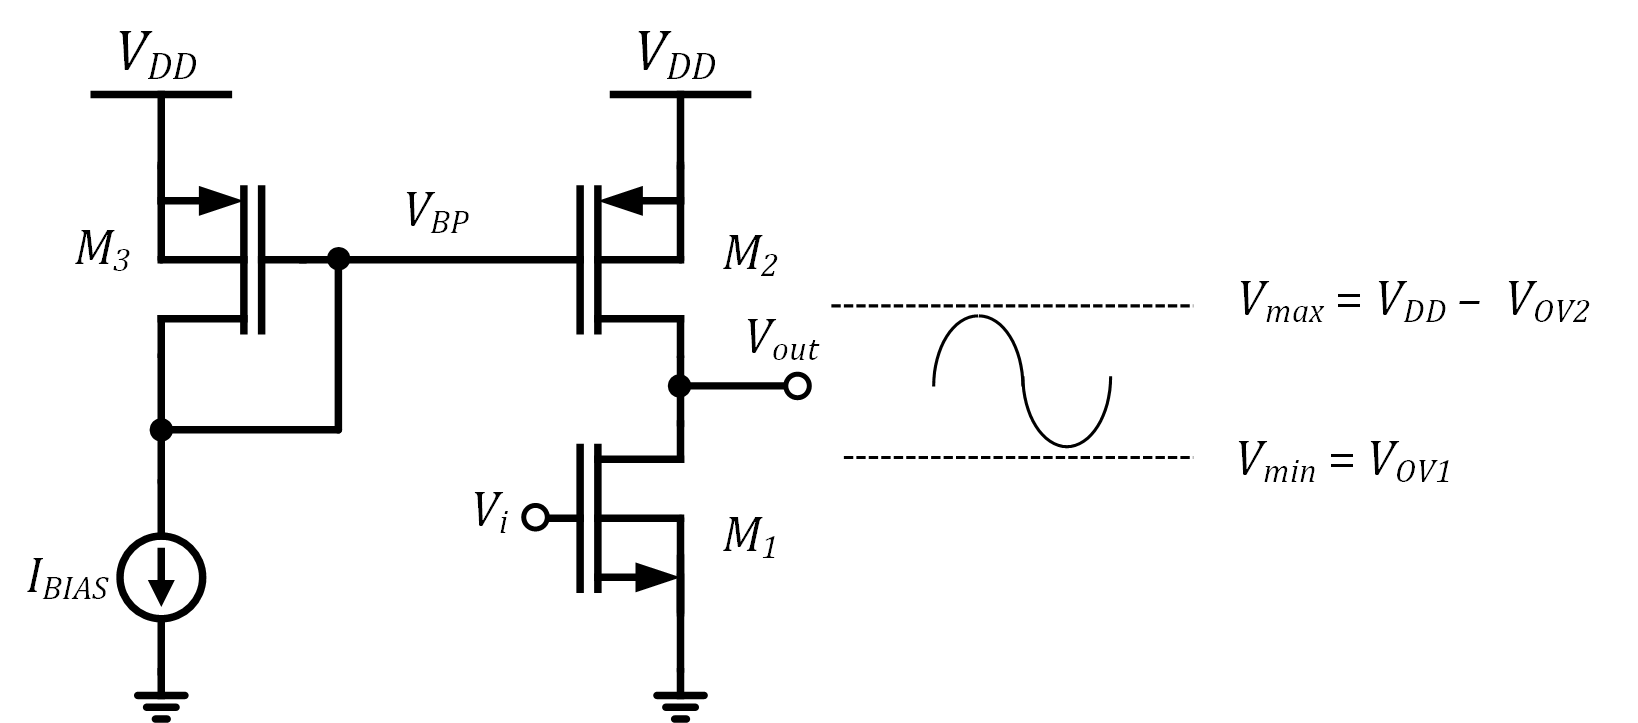
\includegraphics{CS_active_swing.png}
\caption{CS\_active\_swing.png}
\end{figure}

    \begin{align}
V_{swing} &= V_{max} - V_{min}\\
&= V_{DD} - V_{OV2} - V_{OV1}\\
&\approx \boxed{ V_{DD} - 2V_{OV} }
\end{align}

    \begin{itemize}
\item
  The output swing of a common source stage is \(V_{DD} – 2V_{OV}\)
\item
  Common source amplifier thus requires an ``overhead'' of \(2V_{OV}\)
\item
  This structure is often used where wide output swing is required
\end{itemize}

    \hypertarget{output-swing-cs-with-source-degenerated-load}{%
\subsection{Output swing: CS with source-degenerated
load}\label{output-swing-cs-with-source-degenerated-load}}

    \begin{figure}
\centering
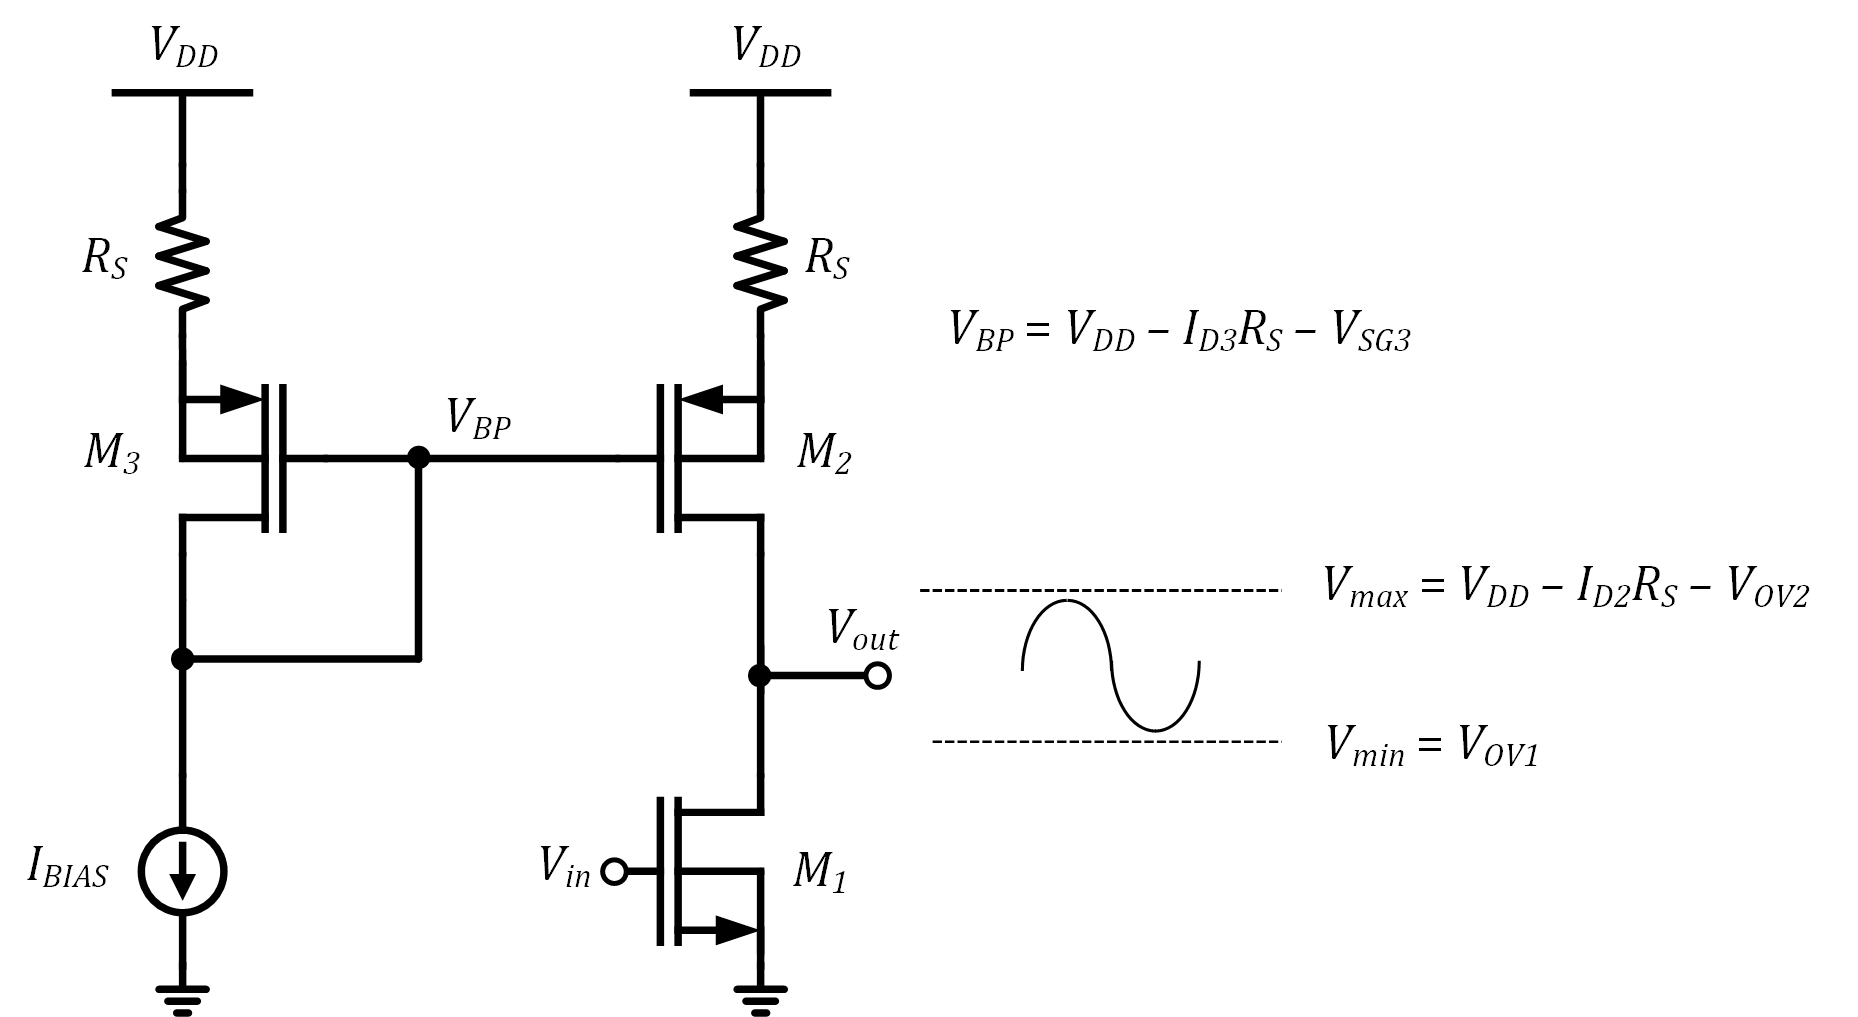
\includegraphics{CS_degenerated_load_swing.png}
\caption{CS\_degenerated\_load\_swing.png}
\end{figure}

    \begin{align}
V_{swing} &= V_{max} - V_{min}\\
&= V_{DD} - I_{D2}R_S - V_{OV2} - V_{OV1}\\
&\approx \boxed{ V_{DD} - I_{D2}R_S - 2V_{OV} }
\end{align}

    \begin{itemize}
\item
  Degenerated load adds \(I_D R_S\) overhead
\item
  Overhead depends on value of \(R_S\), as does \(R_o\) (tradeoff
  between gain and headroom)
\item
  Simple structure, only requires the addition of resistors but no
  additional bias transistors
\end{itemize}

    \hypertarget{output-swing-cascode-amplifier}{%
\subsection{Output swing: cascode
amplifier}\label{output-swing-cascode-amplifier}}

    \begin{figure}
\centering
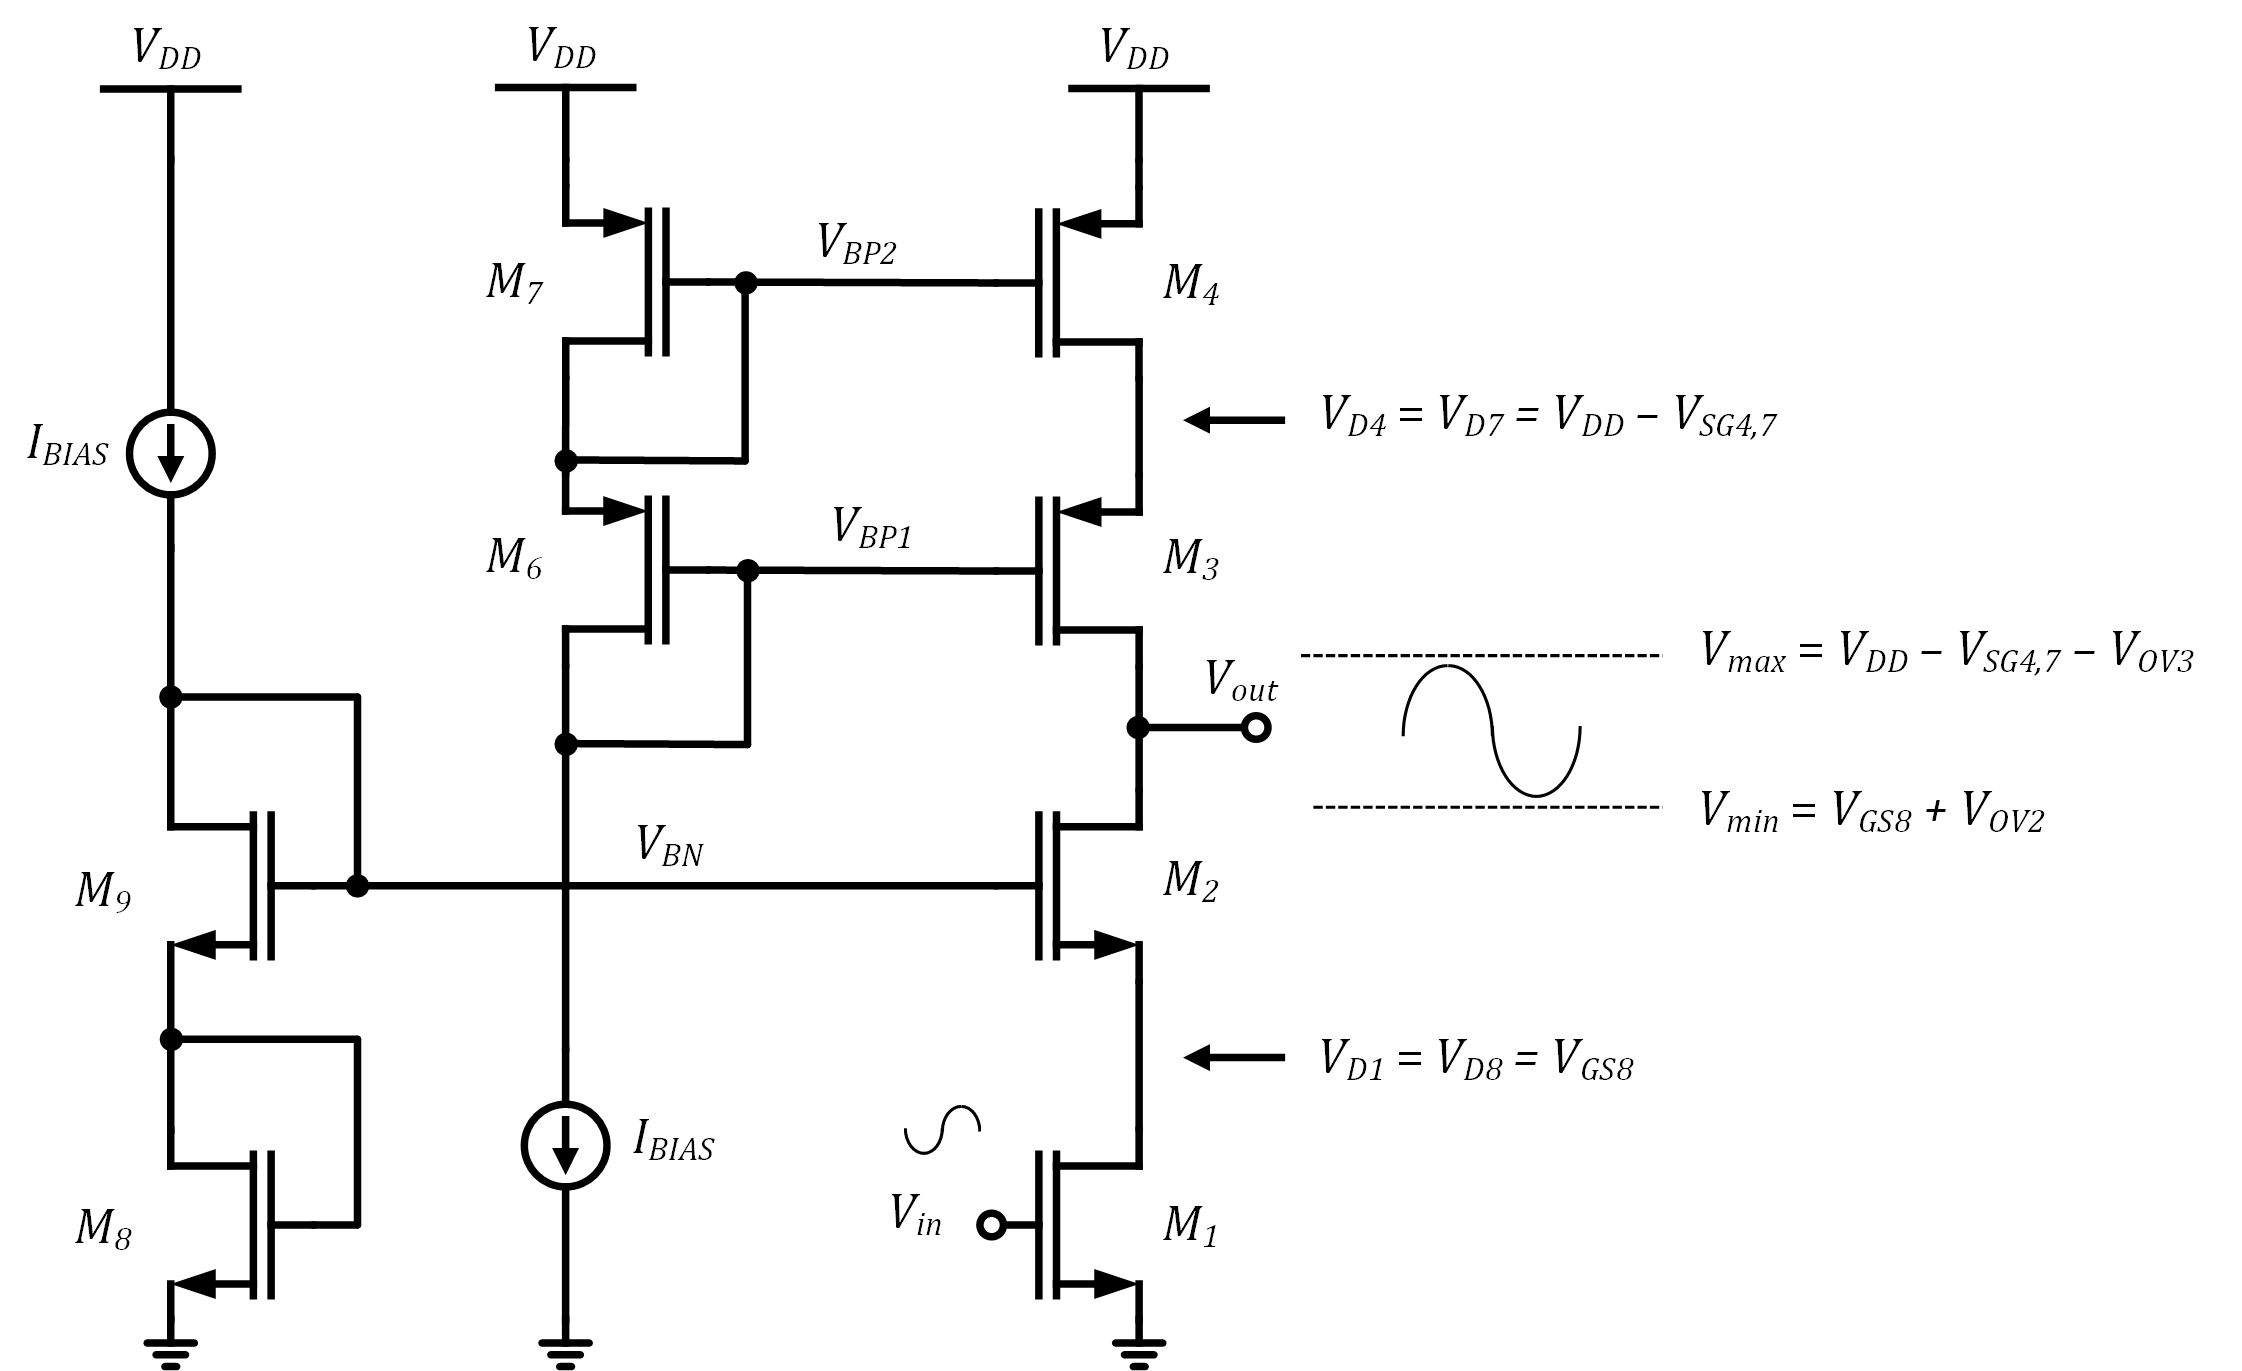
\includegraphics{cascode_amplifier_swing.png}
\caption{cascode\_amplifier\_swing.png}
\end{figure}

    \begin{align}
V_{swing} &= V_{max} - V_{min}\\
&= V_{DD} - V_{SG,4,7} - V_{OV3} - V_{GS8} - V_{OV2}\\
&\approx \boxed{ V_{DD} - 2V_{GS} - 2V_{OV} }
\end{align}

    \begin{itemize}
\item
  Diode-connections of \(M_7\) and \(M_8\) add \(V_{SG}\), \(V_{GS}\)
  overhead
\item
  \(V_{GS} \geq V_{th}\), typically, so headroom depends on device
  threshold(s)
\item
  Need a means of biasing the cascode amplifier that uses less headroom
\end{itemize}

    \hypertarget{biasing-of-mos-circuits}{%
\subsection{Biasing of MOS circuits}\label{biasing-of-mos-circuits}}

    \begin{itemize}
\item
  Design of MOS circuits involves selection of drain currents and aspect
  ratios (\(W/L\)) for all devices in a circuit
\item
  The combination of drain current and \(W/L\) determines the
  \emph{current density} of each device, \$I\_D/W \$, which in turn sets
  the overdrive voltage \(V_{OV}\)
\item
  For example, if we ignore channel-length modulation MOS drain current
  is given by
\end{itemize}

\begin{equation}
I_D \approx \dfrac{1}{2}\mu C_{ox} \dfrac{W}{L}V_{OV}^2
\end{equation}

\begin{itemize}
\tightlist
\item
  Assuming a constant value for \(L\), this results in a direct
  dependence of overdrive on drain current density
\end{itemize}

\begin{equation}
V_{OV} = \sqrt{\dfrac{2I_D}{\mu C_{ox} \dfrac{W}{L}}} = \sqrt{\dfrac{I_D}{W}\cdot\dfrac{2L}{\mu C_{ox}}}
\end{equation}

\begin{itemize}
\tightlist
\item
  As a result, the voltage headroom (i.e.~swing) of a circuit is
  determined by the current densities of transistors in the signal path
\end{itemize}

    \hypertarget{simple-current-reference}{%
\subsection{Simple current reference}\label{simple-current-reference}}

    \begin{figure}
\centering
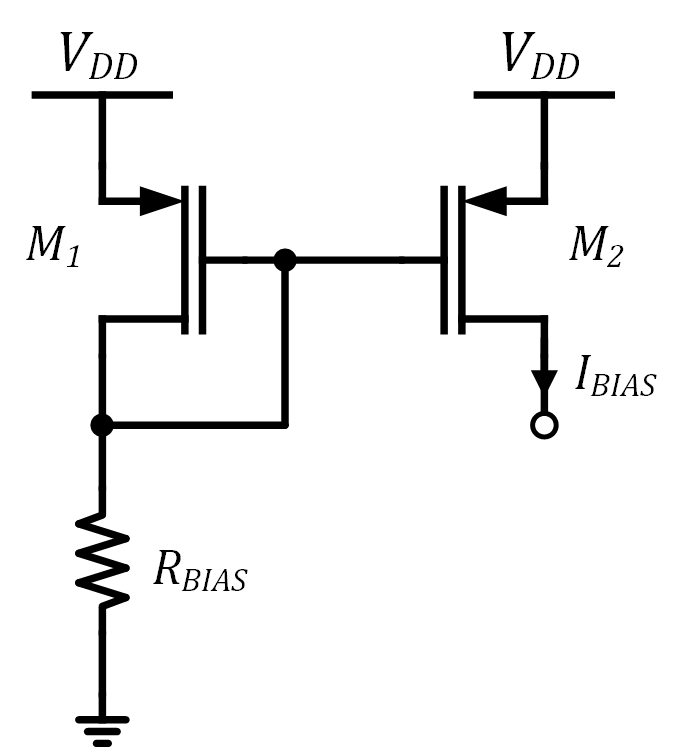
\includegraphics{simple_current_reference.png}
\caption{simple\_current\_reference.png}
\end{figure}

    \begin{itemize}
\tightlist
\item
  The current in \(M_1\) is set by the voltage drop across \(R_{BIAS}\)
\end{itemize}

\begin{equation}
I_{D1} = \dfrac{V_{DD}-V_{SG1}}{R_{BIAS}}
\end{equation}

\begin{itemize}
\tightlist
\item
  \(V_{SG}\) of \(M_1\) is given by
\end{itemize}

\begin{equation}
V_{SG1} = |V_{thp}| + \sqrt{\dfrac{2I_{D1}}{\mu_p C_{ox}\left(\frac{W}{L}\right)_1}}
\end{equation}

    \begin{itemize}
\item
  A simple current reference can be created using a diode-connected MOS
  device in series with a resistance between \(V_{DD}\) and ground
\item
  However, variations in (primarily) \(V_{DD}\), \(V_{thp}\), and
  \(R_{BIAS}\) result in an \(I_{BIAS}\) that vary significantly with
  manufacturing (process) and temperature
\item
  These variations are collectively known as ``PVT'' (process, voltage,
  temperature), and significant effort is invested in making analog
  circuits robust against these sources of variability
\end{itemize}

    \hypertarget{supply-independent-reference}{%
\subsection{Supply-independent
reference}\label{supply-independent-reference}}

    \begin{figure}
\centering
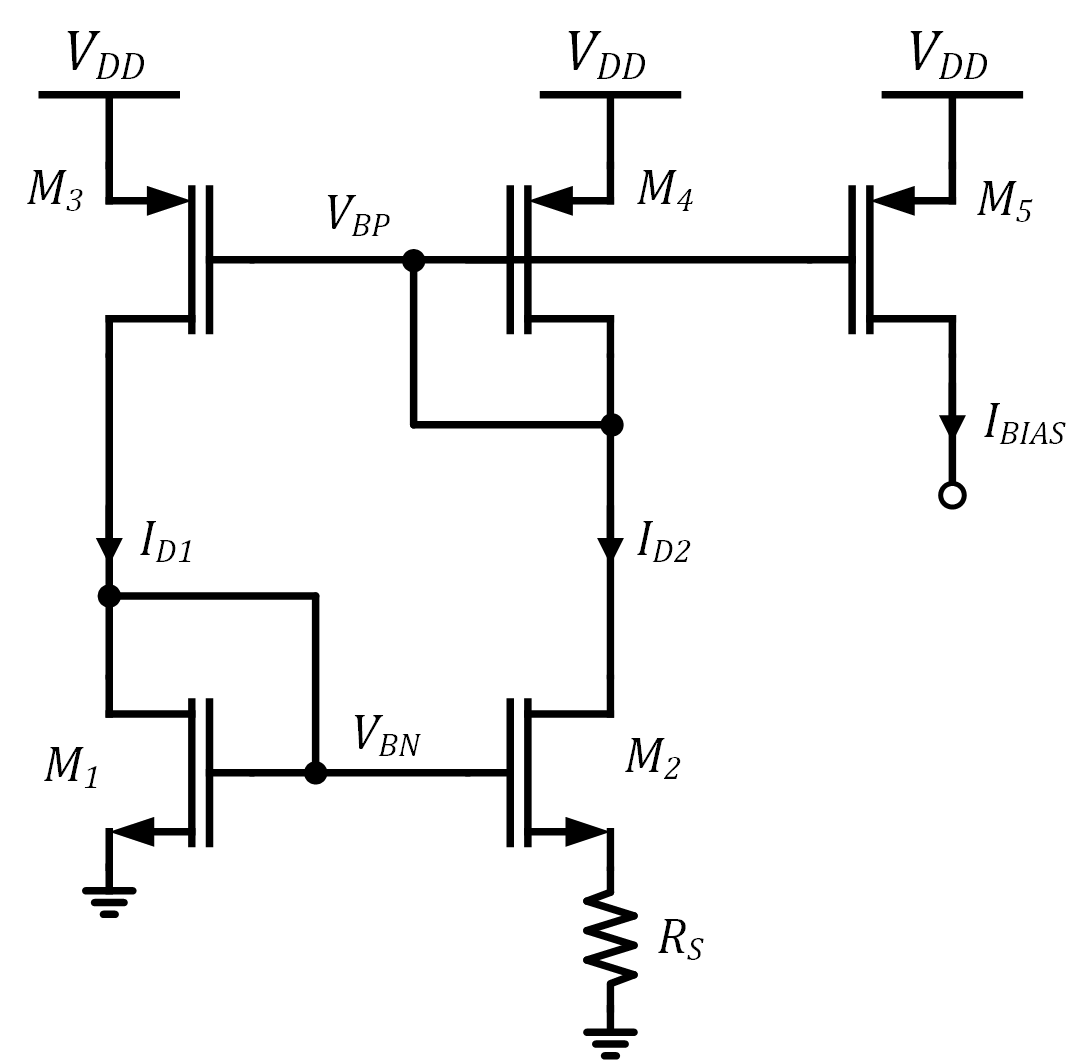
\includegraphics{current_reference.png}
\caption{current\_reference.png}
\end{figure}

    \begin{itemize}
\item
  A more reliable means of generating bias currents involves
  ``self-biased,'' supply-independent reference circuits
\item
  In the circuit depicted here, often called a ``constant \(g_m\)''
  reference, \(I_{D2}\) is given by
\end{itemize}

\begin{equation}
I_{D2} = \dfrac{V_{S2}}{R_S} = \dfrac{V_{BN}-V_{GS2}}{R_S} = \dfrac{V_{GS1}-V_{GS2}}{R_S} = \dfrac{\Delta V_{GS}}{R_S}
\end{equation}

\begin{itemize}
\tightlist
\item
  \(\Delta V_{GS}\) depends on the ratio of \((W/L)_2\) to \((W/L)_1\),
  which is independent of \(V_{DD}\)
\end{itemize}

    \hypertarget{cascode-current-mirror}{%
\subsection{Cascode current mirror}\label{cascode-current-mirror}}

    \begin{figure}
\centering
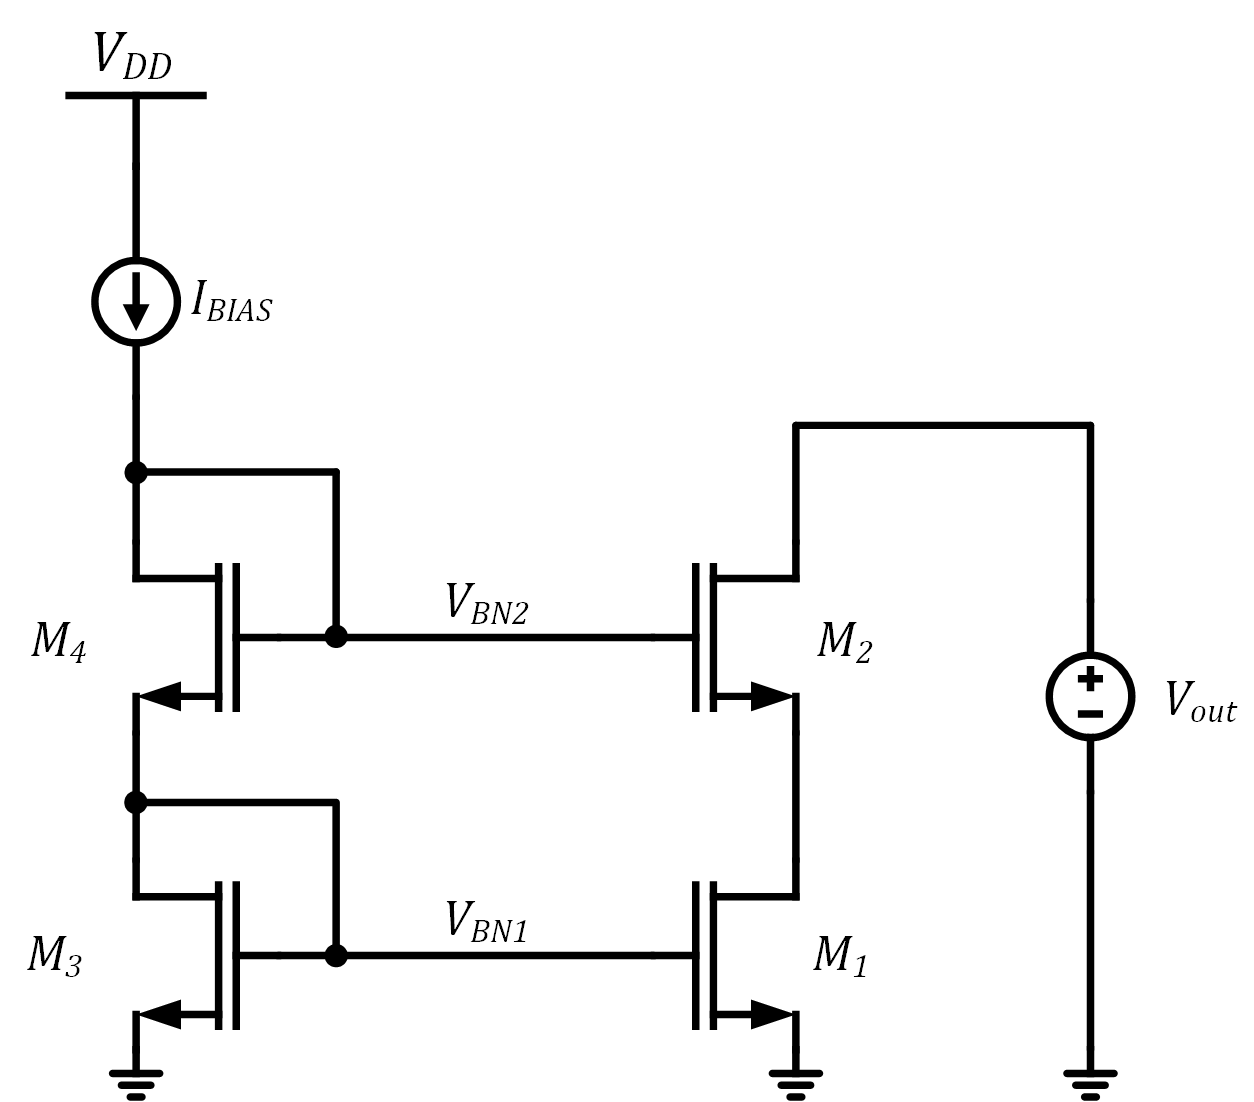
\includegraphics{cascode_current_mirror.png}
\caption{cascode\_current\_mirror.png}
\end{figure}

    \begin{itemize}
\tightlist
\item
  Assuming \(I_{D1} = I_{D3}\), we can write
\end{itemize}

\begin{equation}
V_{S2} = V_{D1} = V_{GS3} = V_{GS1}
\end{equation}

\begin{itemize}
\tightlist
\item
  To keep \(M_2\) in saturation, \(V_{out}\) needs to satisify
\end{itemize}

\begin{equation}
V_{out} - V_{S2} > V_{GS2} - V_{th2} 
\end{equation}

\begin{itemize}
\tightlist
\item
  This sets the minimum value of \(V_{out}\) to be
\end{itemize}

\begin{equation}
V_{out} > V_{GS1} + V_{GS2} - V_{th2} = V_{GS1} + V_{OV2}
\end{equation}

    \begin{itemize}
\item
  Cascode current mirrors are employed everywhere high precision (or
  high gain) is needed
\item
  However, the basic cascode current mirror has a headroom problem,
  because \(V_{out}\) needs to be greater than \(2V_{OV}\) to ensure
  saturation for both \(M_1\) and \(M_2\)
\item
  To improve upon this, we need to modify the approach used to generate
  \(V_{BN1}\) and \(V_{BN2}\)
\end{itemize}

    \hypertarget{low-voltage-cascode-bias}{%
\subsection{Low-voltage cascode bias}\label{low-voltage-cascode-bias}}

    \begin{figure}
\centering
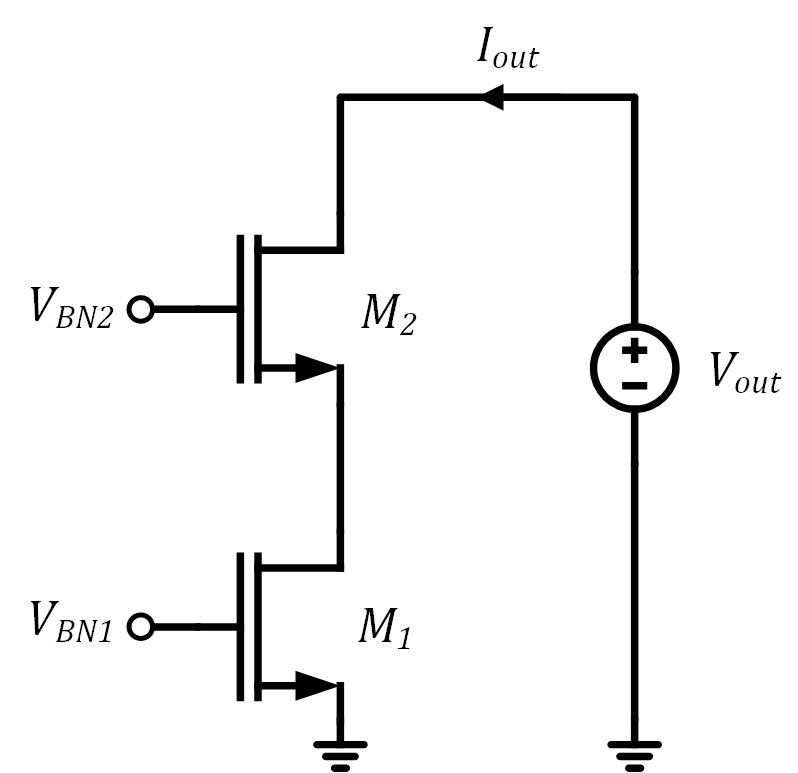
\includegraphics{cascode_current_source.png}
\caption{cascode\_current\_source.png}
\end{figure}

    \begin{itemize}
\tightlist
\item
  To minimize the headroom required by the cascode current source,
  \(M_2\) should be biased such that
\end{itemize}

\begin{equation}
V_{S2} = V_{D1} \approx V_{OV1}
\end{equation}

\begin{itemize}
\tightlist
\item
  We can achieve this by selecting a value for \(V_{BN2}\) that
  satisfies
\end{itemize}

\begin{equation}
V_{BN2} = V_{OV1} + V_{GS2}
\end{equation}

\begin{itemize}
\tightlist
\item
  In this case, the minimum output voltage would be given by
\end{itemize}

\begin{equation}
V_{out} > V_{OV1} + V_{OV2} \approx 2V_{OV}
\end{equation}

\begin{itemize}
\tightlist
\item
  How can we generate \(V_{BN1}\) and \(V_{BN2}\) to achieve this?
\end{itemize}

    \hypertarget{generation-of-vbn1}{%
\subsection{Generation of VBN1}\label{generation-of-vbn1}}

    \begin{figure}
\centering
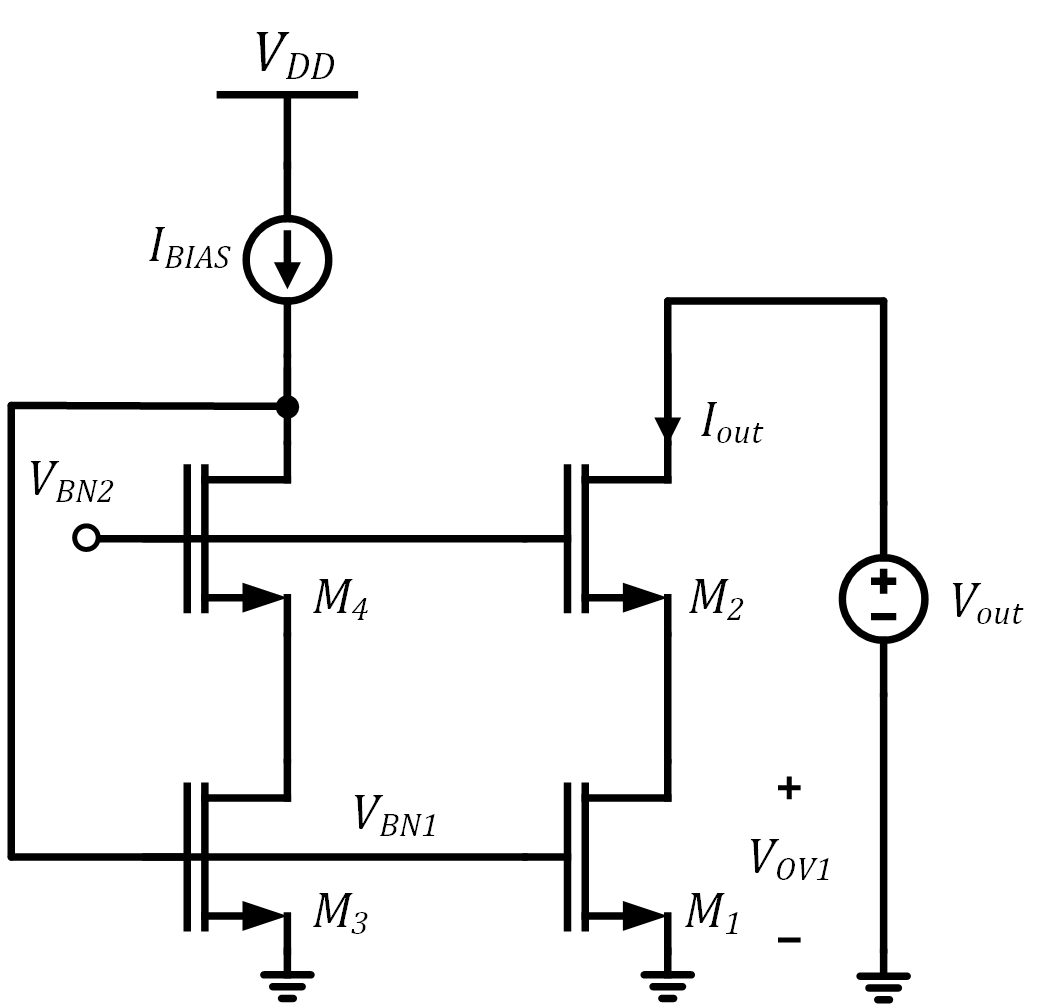
\includegraphics{cascode_VBN1.png}
\caption{cascode\_VBN1.png}
\end{figure}

    \begin{itemize}
\item
  \(V_{BN1}\) is generated by diode-connecting \(M_3\) (\(M_3\) and
  \(M_1\) form a current mirror)
\item
  The presence of \(M_4\) does not affect the value of \(V_{BN1}\), but
  \(V_{BN1}\) needs to be high enough to keep \(M_4\) in saturation
\item
  Our goal is to select a value of \(V_{BN2}\) that is high enough to
  keep \(M_1\) (\(M_3\)) in saturation, but no higher than this
\item
  Once again, if we assume that the drain voltage of \(M_1\) is
  \emph{exactly} equal to \(V_{OV1}\), the minimum value of \(V_{out}\)
  will be \(V_{OV1} + V_{OV2}\)
\item
  The value of \(V_{BN2}\) that achieves this is
\end{itemize}

\begin{equation}
V_{BN2} = V_{OV1} + V_{GS4}
\end{equation}

    \hypertarget{generation-of-vbn2}{%
\subsection{Generation of VBN2}\label{generation-of-vbn2}}

    \begin{figure}
\centering
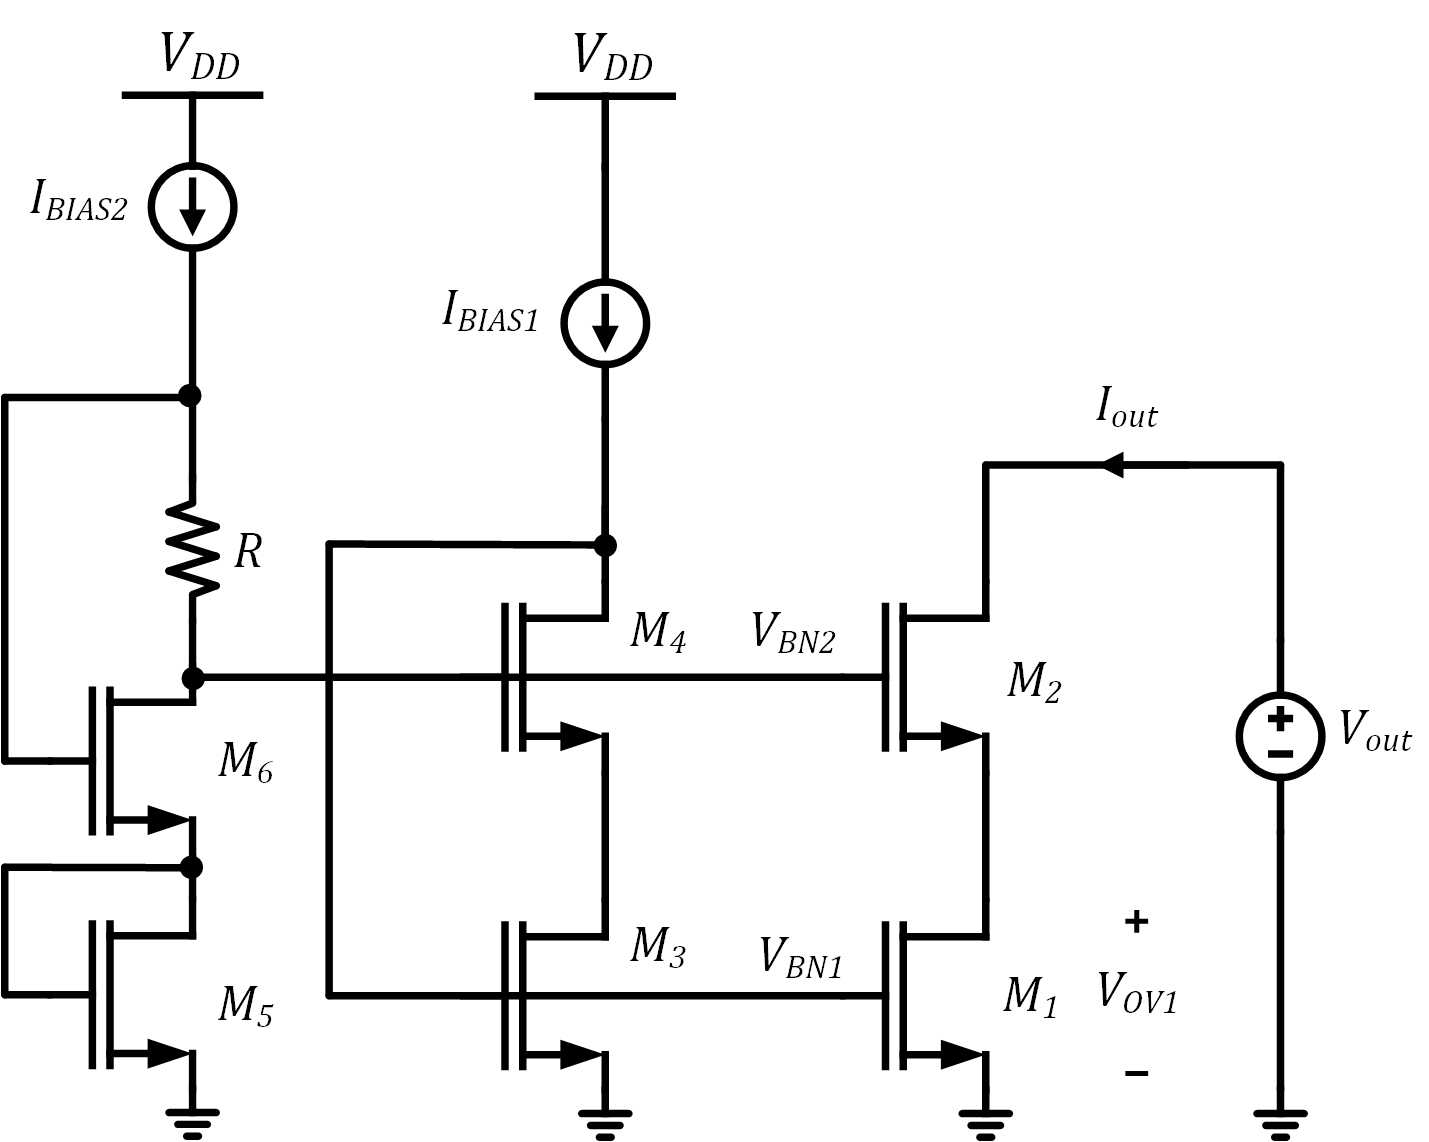
\includegraphics{cascode_VBN2_a.png}
\caption{cascode\_VBN2\_a.png}
\end{figure}

    \begin{itemize}
\item
  One method of generating \(V_{BN2}\) is shown here
\item
  Remember, we just need to ensure that
\end{itemize}

\begin{equation}
V_{BN2} = V_{OV1} + V_{GS2}
\end{equation}

\begin{itemize}
\tightlist
\item
  To achieve this, we note that
\end{itemize}

\begin{equation}
V_{BN2} = V_{GS5} + V_{GS6} - I_{BIAS2}\cdot R
\end{equation}

\begin{itemize}
\tightlist
\item
  This results in the following condition for the resistance \(R\)
\end{itemize}

\begin{align}
R &= \dfrac{V_{GS5} + V_{GS6} - V_{BN2} }{I_{BIAS2}} = \dfrac{V_{GS5} + V_{GS6} - V_{OV1} - V_{GS2} }{I_{BIAS2}}
\end{align}

\begin{itemize}
\tightlist
\item
  If all values of \(V_{GS}\) are considered to be approximately equal,
  this results in
\end{itemize}

\begin{equation}
R \approx \dfrac{V_{thn}}{I_{BIAS2}}
\end{equation}

    \hypertarget{low-overhead-pmos-cascode-bias}{%
\subsection{Low-overhead PMOS cascode
bias}\label{low-overhead-pmos-cascode-bias}}

    \begin{figure}
\centering
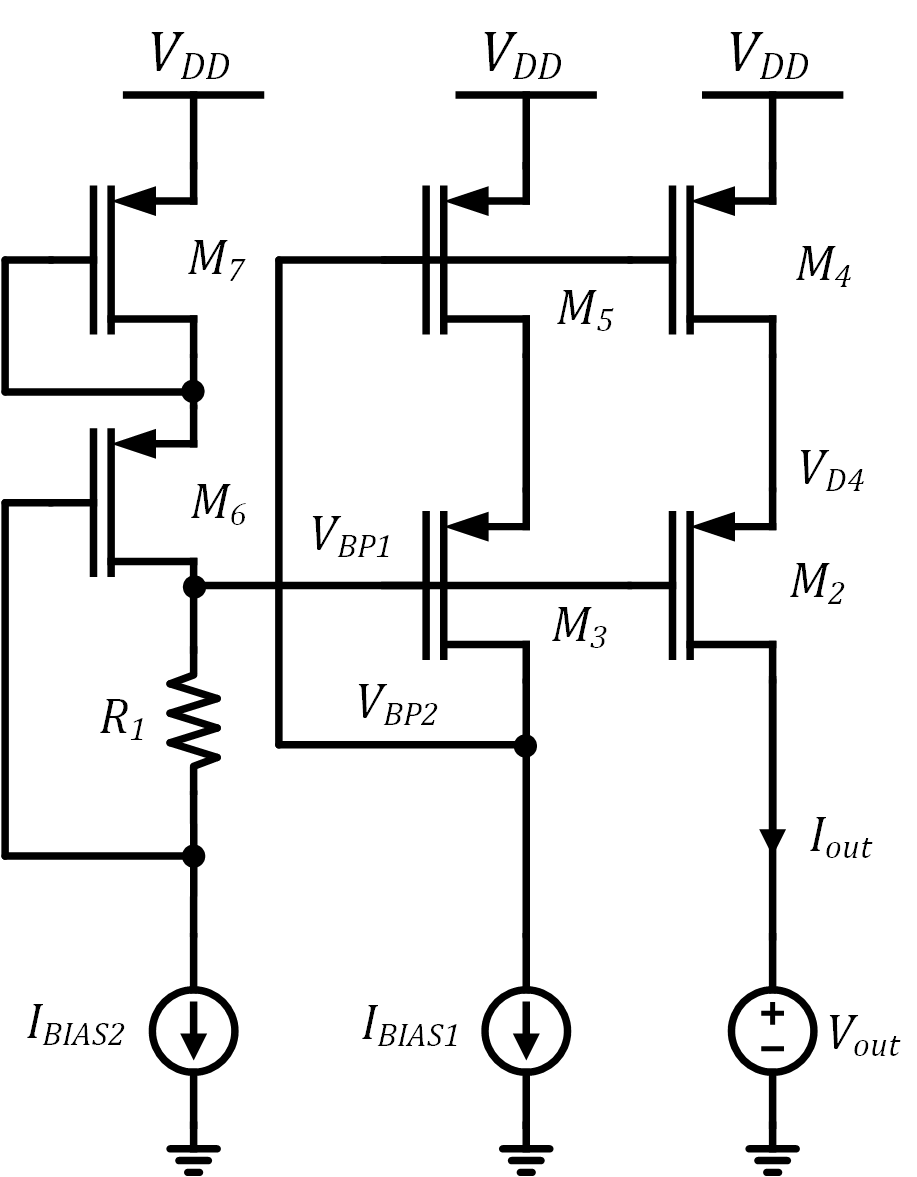
\includegraphics{PMOS_cascode_bias.png}
\caption{PMOS\_cascode\_bias.png}
\end{figure}

    \begin{itemize}
\tightlist
\item
  To guarantee saturation for \(M_2\) and \(M_4\) and use minimal
  headroom, we need to ensure that
\end{itemize}

\begin{equation}
V_{BP1} \approx V_{DD} - V_{OV4} - V_{SG2}
\end{equation}

\begin{itemize}
\tightlist
\item
  As with the \(NMOS\) version of the circuit, the above expression
  needs to be related to the following
\end{itemize}

\begin{equation}
V_{BP1} = V_{DD} - V_{SG7} - V_{SG6} + I_{BIAS2}\cdot R_1
\end{equation}

\begin{itemize}
\tightlist
\item
  Equation the two results in an expression for \(R_1\) that we can use
  for design:
\end{itemize}

\begin{equation}
R_1 = \dfrac{V_{SG7}+V_{SG6}-V_{SG2}-V_{OV4}}{I_{BIAS2}}
\end{equation}

    \hypertarget{alternate-realization-of-vbn2-self-biased-cascode}{%
\subsection{Alternate realization of VBN2 (self-biased
cascode)}\label{alternate-realization-of-vbn2-self-biased-cascode}}

    \begin{figure}
\centering
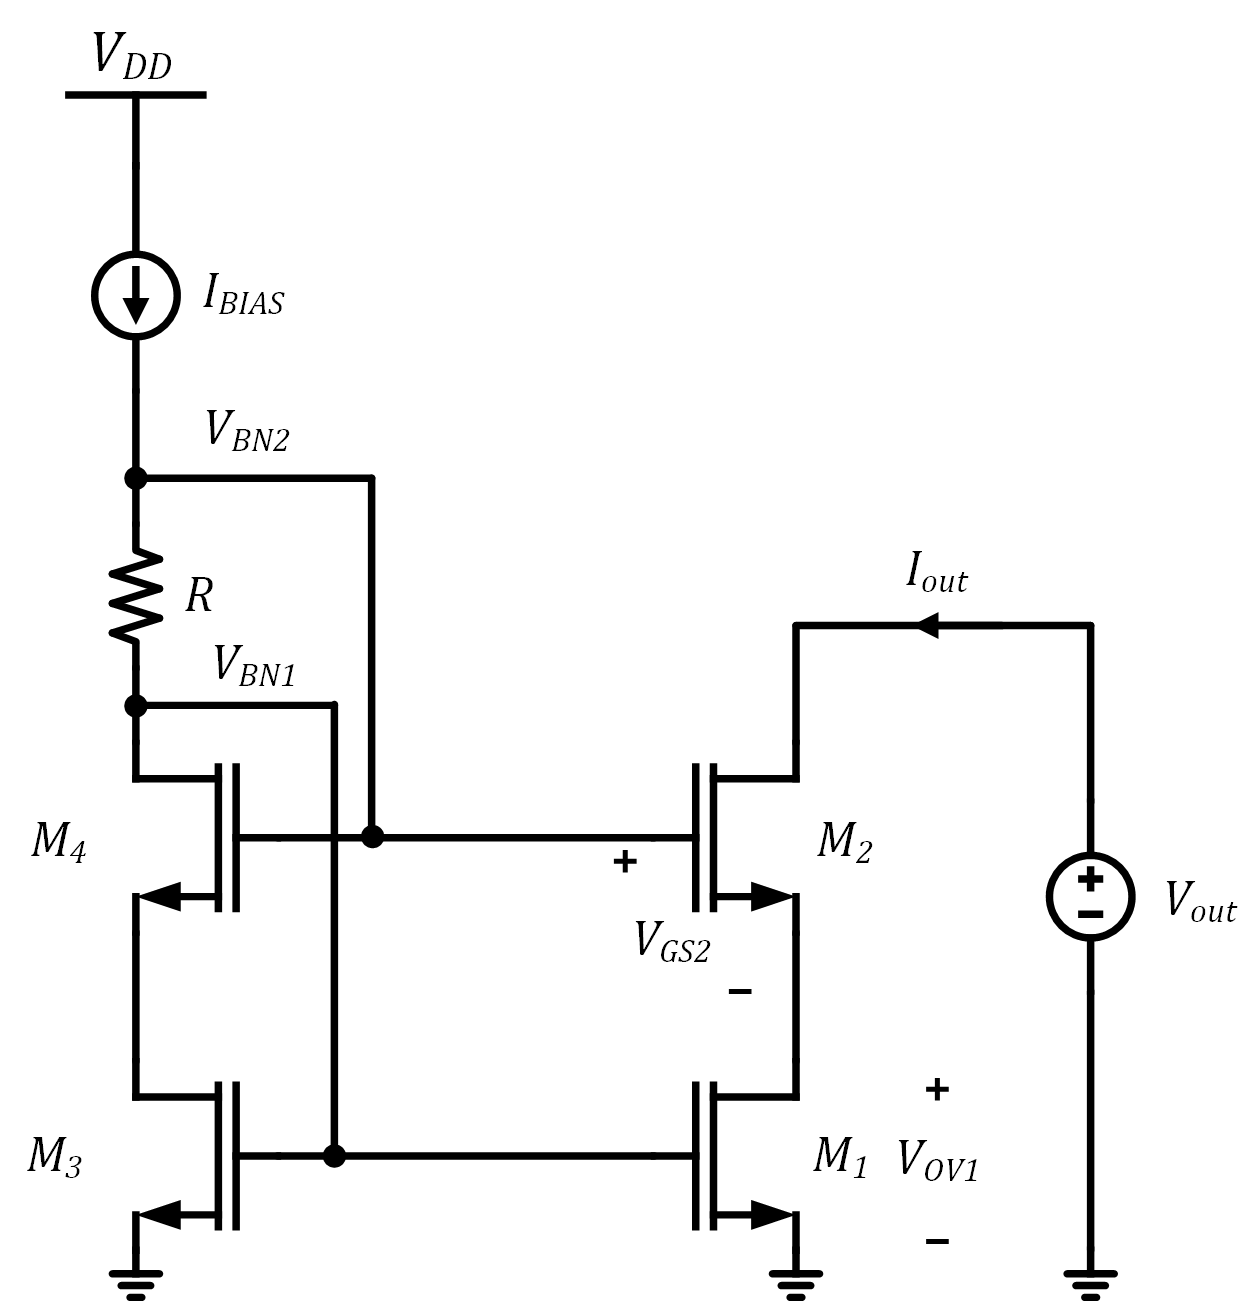
\includegraphics{cascode_self_biased.png}
\caption{cascode\_self\_biased.png}
\end{figure}

    \begin{itemize}
\item
  One disadvantage of the previous biasing schemes is the need for an
  extra current branch, which increases power and cirucuit area
\item
  The configuration here generates \(V_{BN1}\) and \(V_{BN2}\) without
  the additional current branch
\item
  \(R\) should be selected such that
\end{itemize}

\begin{equation}
V_{BN1} + I_{BIAS}\cdot R = V_{OV1} + V_{GS2}
\end{equation}

\begin{itemize}
\tightlist
\item
  This results in
\end{itemize}

\begin{equation}
R = \dfrac{V_{GS2} - V_{th1}}{I_{BIAS}}
\end{equation}

\begin{itemize}
\item
  Assuming \(V_{th1} \approx V_{th2}\), the voltage drop across \(R\) is
  equal to the overdrive voltage of \(M_{2,4}\) (say,
  \textasciitilde{}\(200mV\))
\item
  Note that resistance and \(MOS\) parameters will vary differently due
  to process and temperature, so \(R\) should be selected to take this
  into account (simulations required)
\end{itemize}

    \hypertarget{loading-effects}{%
\subsection{Loading effects}\label{loading-effects}}

    \begin{figure}
\centering
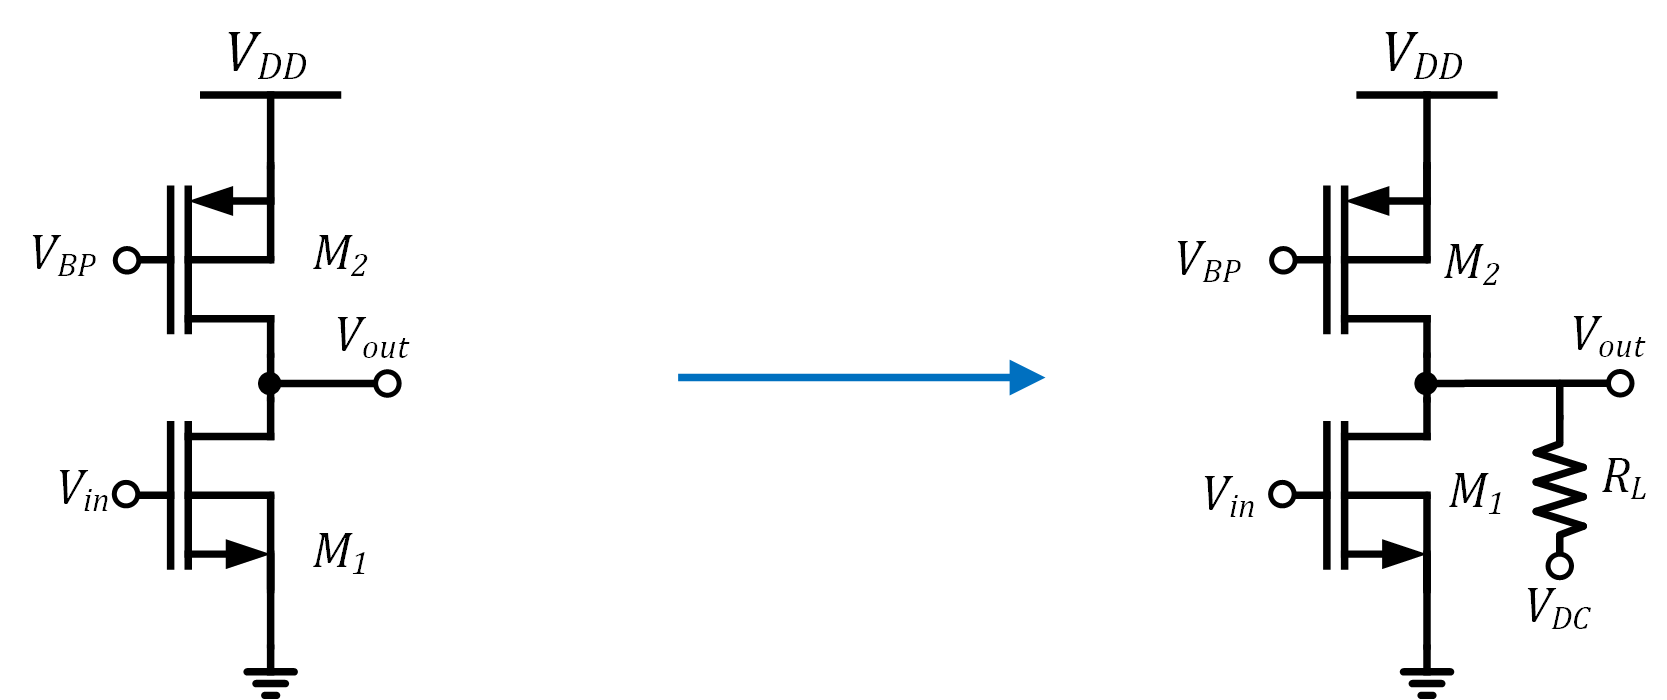
\includegraphics{CS_loading.png}
\caption{CS\_loading.png}
\end{figure}

    \begin{itemize}
\item
  Gain in common-source (and related structures) is achieved with high
  output resistance
\item
  In our Level 1 process model, the output resistance of a cascode
  amplifier with \(1mA\) bias current is roughly \(500k\Omega\)
  (\(g_m r_o^2/2\))
\item
  If \(R_L << R_o\), the gain is reduced to approximately \(g_{m1}R_L\)
\item
  Load resistance (e.g.~in an opamp feedback network) decreases the gain
  of these amplifiers, an effect referred to as \emph{loading}
\end{itemize}

    \hypertarget{source-follower-stage}{%
\subsection{Source follower stage}\label{source-follower-stage}}

    \begin{figure}
\centering
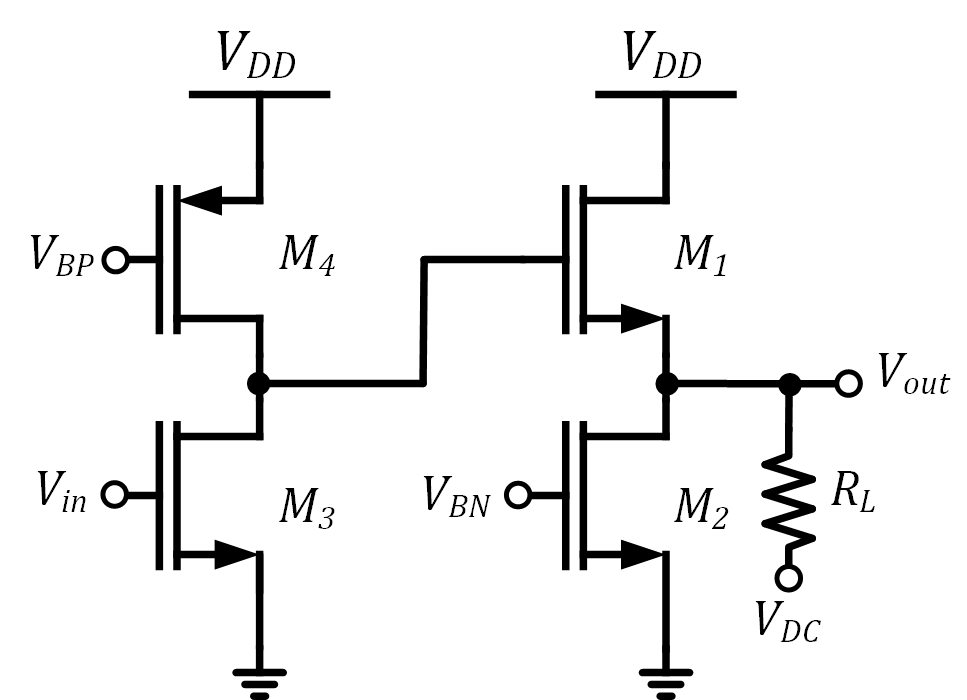
\includegraphics{source_follower_buffer.png}
\caption{source\_follower\_buffer.png}
\end{figure}

    \begin{itemize}
\item
  A source follower stage is often used to isolate/buffer the high
  output resistance of a gain stage from low-valued load resistances
\item
  The output resistance of a source follower stage is approximately
  \(1/g_m\), while the ``gain'' is approximately \(1\)
\item
  Due to the unity gain, we say the output (which is located at the
  source of the \(g_m\) devices) ``follows'' the input at the gate
\end{itemize}

    \hypertarget{source-follower-small-signal-analysis}{%
\subsection{Source-follower small-signal
analysis}\label{source-follower-small-signal-analysis}}

    \begin{figure}
\centering
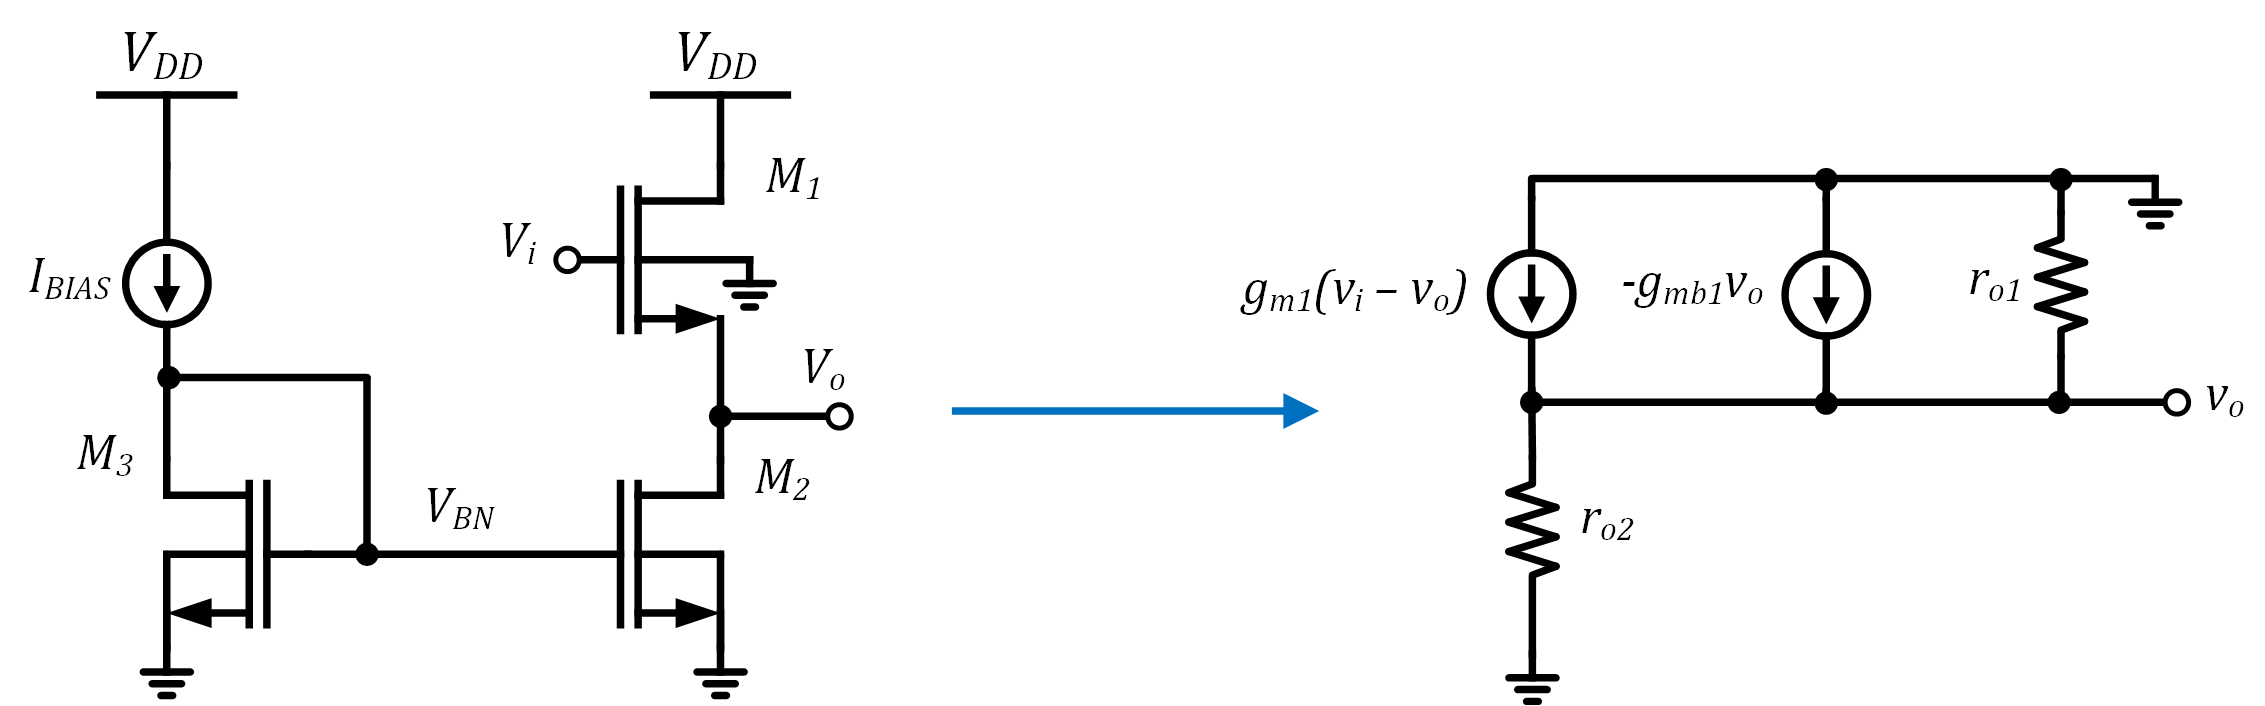
\includegraphics{source_follower_small_signal.png}
\caption{source\_follower\_small\_signal.png}
\end{figure}

    \begin{itemize}
\item
  \(M_1\) constitutes the ``gain'' device, meaning that the signal is
  conveyed via its transconductance \(g_{m1}\)
\item
  The \(DC\) level output voltage is \(V_{GS1}\) lower than that of the
  input voltage, making the minimum value of the input signal
  \(V_{OV2} + V_{GS1}\)
\item
  Body effect is present in \(M_1\), due to the fact that its source is
  not directly connected to ground
\item
  We can again use the Norton equivalent circuit to determine the \(DC\)
  transfer function
\end{itemize}

    \hypertarget{equivalent-transconductance-gm}{%
\subsection{Equivalent transconductance
(Gm)}\label{equivalent-transconductance-gm}}

    \begin{figure}
\centering
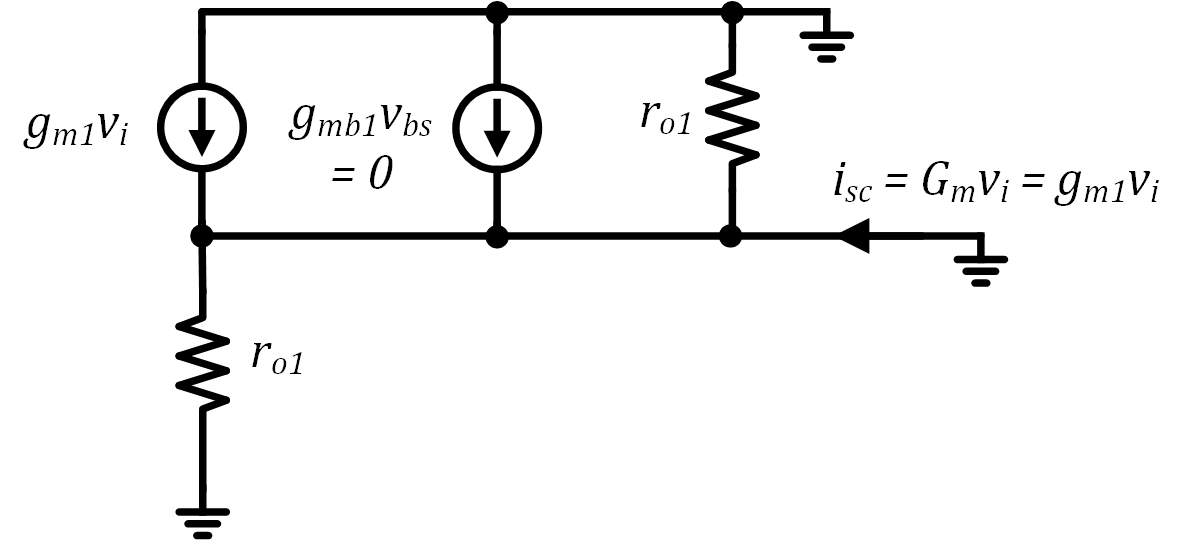
\includegraphics{SF_Gm.png}
\caption{SF\_Gm.png}
\end{figure}

    \begin{align}
G_m &= \dfrac{i_{sc}}{v_i}\\
\\
&= -\dfrac{g_{m1}\cdot v_i}{v_i} = \boxed{ -g_{m1} }
\end{align}

    \begin{itemize}
\tightlist
\item
  For determination of \(G_m\), we short-circuit the output and use the
  ratio of \(i_{sc}\) to \(v_i\)
\item
  The \(g_{mb}\), \(r_{o1}\), and \(r_{o2}\) contributions to \(i_{sc}\)
  disappear (i.e.~they do not contribute), since
  \(v_{sb1} = v_{ds1} = v_{ds2} = 0\)
\item
  As with the common-source amplifier, the equivalent transconductance
  \(G_m\) is equal to \(g_{m1}\), but the polarity is reversed (i.e.~the
  source-follower is a non-inverting structure)
\end{itemize}

    \hypertarget{equivalent-resistance-ro}{%
\subsection{Equivalent resistance (Ro)}\label{equivalent-resistance-ro}}

    \begin{figure}
\centering
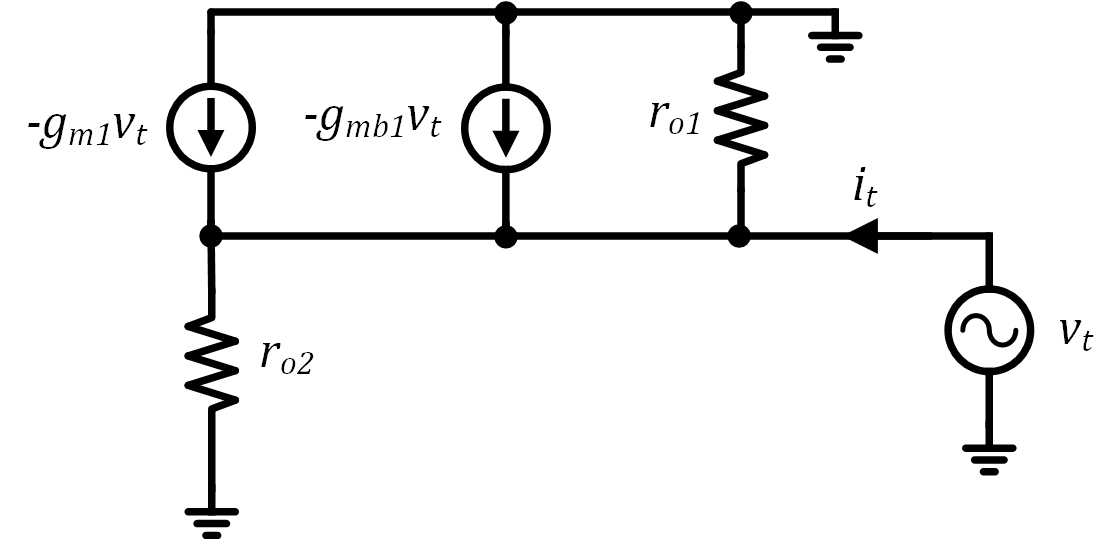
\includegraphics{SF_Ro.png}
\caption{SF\_Ro.png}
\end{figure}

    \begin{itemize}
\tightlist
\item
  The ``test current'' \(i_t\) is the sum of contributions from
  \(r_{o1}\), \(r_{o2}\) and \(g_{m1}\), \(g_{mb1}\)
\end{itemize}

\begin{align}
i_t &= \dfrac{v_t}{r_{o1}} + (g_{mb1} + g_{m1})v_t + \dfrac{v_t}{r_{o2}}\\
\end{align}

\begin{itemize}
\tightlist
\item
  Because each contribution has a linear relationship with \(v_t\), the
  equivalent output resistance can be expressed as the parallel
  combination of 4 individual resistances
\end{itemize}

\begin{align}
R_o &= \dfrac{v_t}{i_t} \\
&= r_{o1}||r_{o2}||\dfrac{1}{g_{m1}}||\dfrac{1}{g_{mb1}}
\end{align}

    \begin{itemize}
\tightlist
\item
  If we make use of the fact that \(g_m r_o >> 1\) for any useful
  \(MOS\) transistor, the output impedance can be approximated as
\end{itemize}

\begin{equation}
R_o = r_{o1}||r_{o2}||\dfrac{1}{g_{m1}}||\dfrac{1}{g_{mb1}} \approx \boxed{ \dfrac{1}{g_{m1} + g_{mb1}} }
\end{equation}

    \hypertarget{source-follower-gain}{%
\subsection{Source follower gain}\label{source-follower-gain}}

    \begin{itemize}
\tightlist
\item
  Using our Norton model approach, the gain is determined as
\end{itemize}

\begin{equation}
A_v = -G_m R_o = g_{m1}\cdot \dfrac{1}{g_{m1} + g_{mb1}}
\end{equation}

\begin{itemize}
\tightlist
\item
  If, for example, \(g_{mb1} = 0.1 g_{m1}\), then \(A_v \approx 0.9\)
\item
  In the ideal case, the source follower provides unity gain while
  presenting a lot output impedance to resistive loads
\item
  Given the relationship between \(g_m\) and drain current \(I_{D1}\),
  we can see that decreasing the output impedance (and thus increasing
  the load driving capability) requires an increase in power
  dissipation:
\end{itemize}

\begin{equation}
\dfrac{1}{g_{m1}} = \dfrac{V_{OV1}}{2I_{D1}}
\end{equation}

    \hypertarget{where-were-headed}{%
\subsection{Where we're headed}\label{where-were-headed}}

    \begin{figure}
\centering
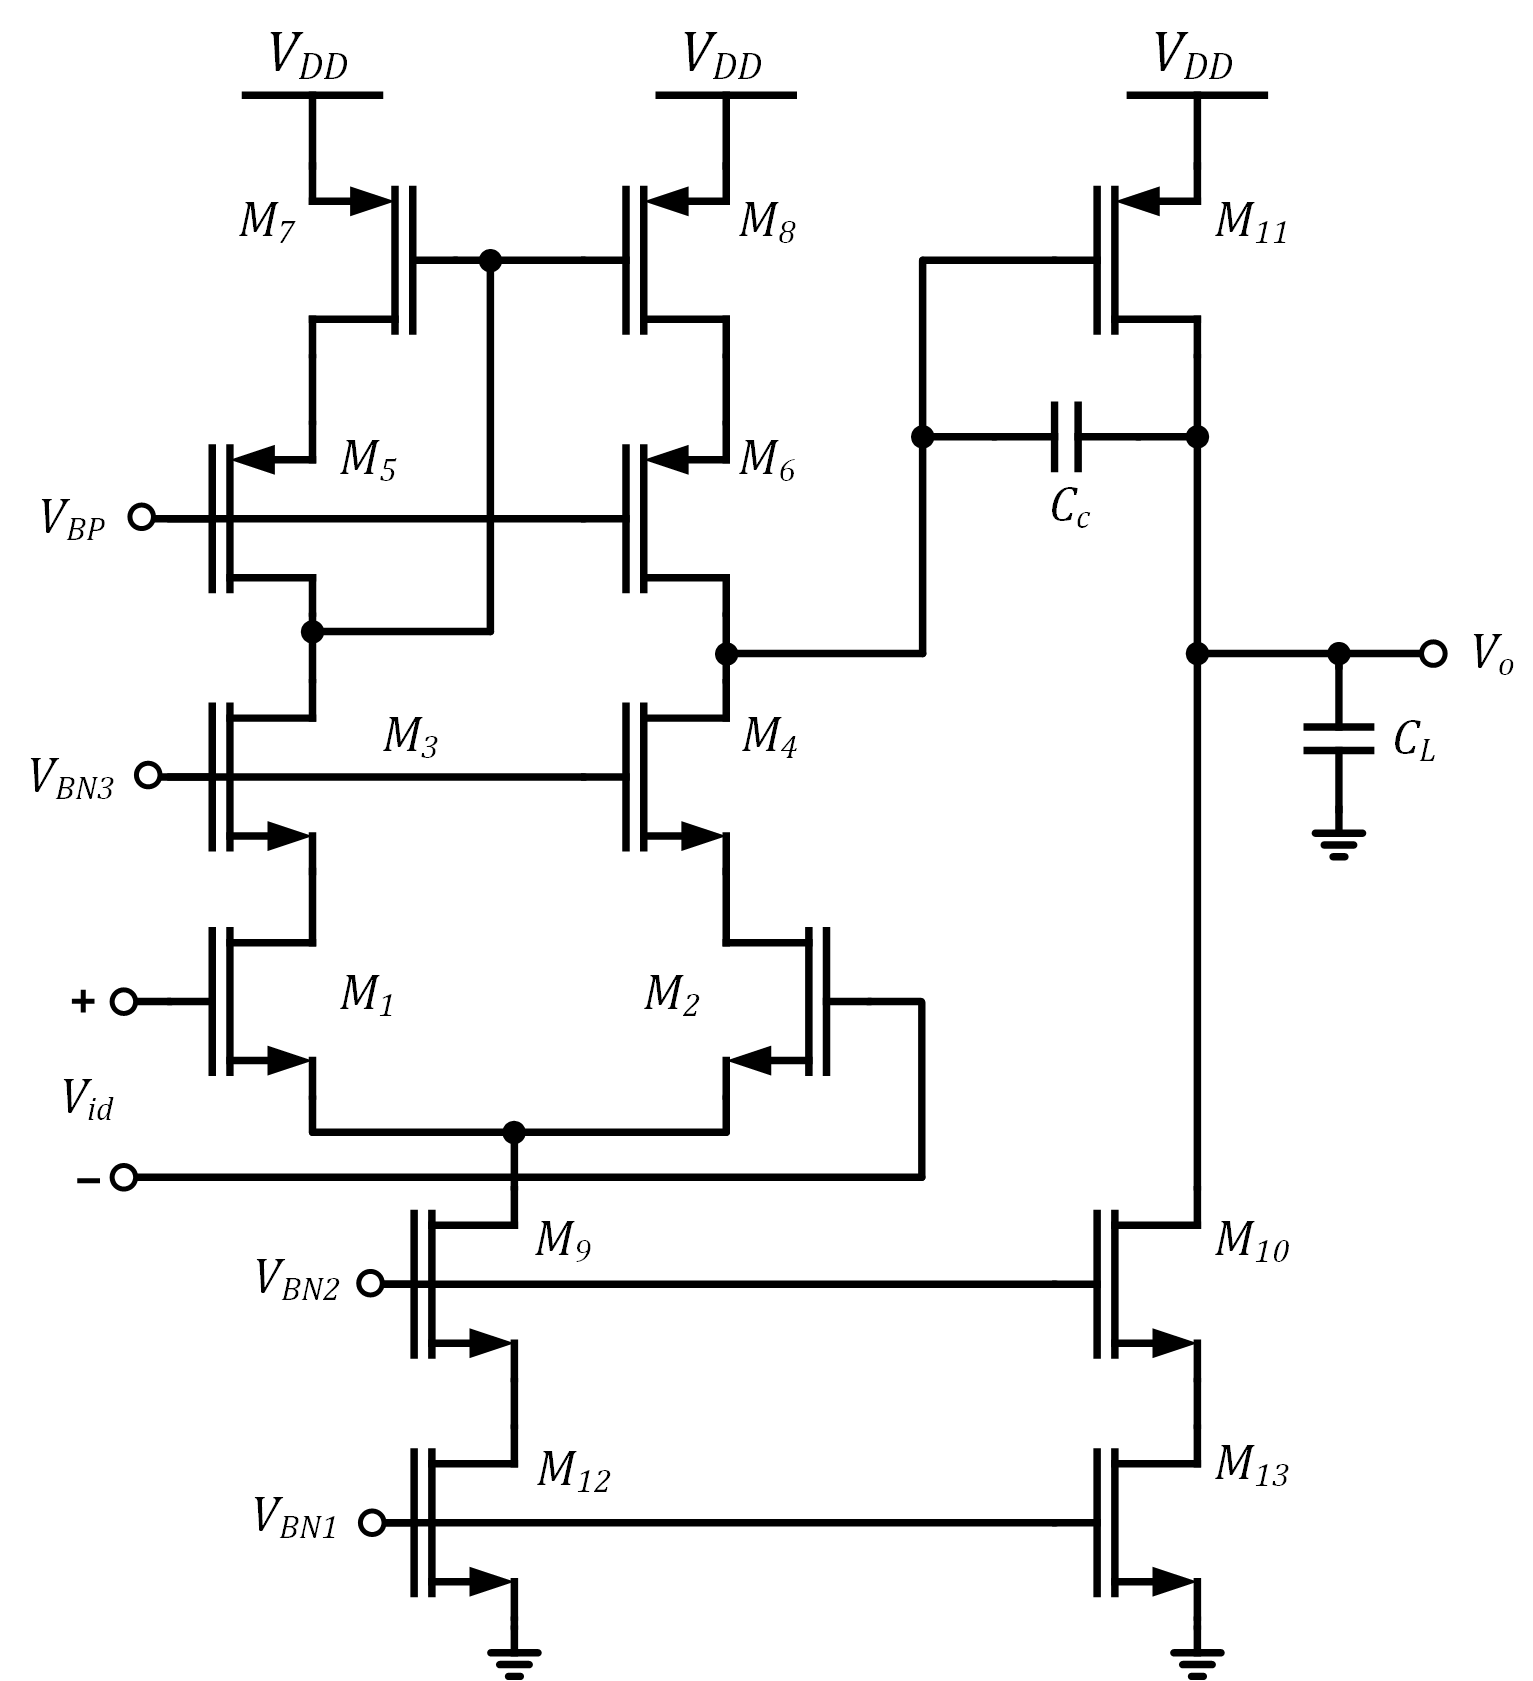
\includegraphics{telescopic_ota.png}
\caption{telescopic\_ota.png}
\end{figure}

    \begin{itemize}
\item
  We want to create a high-gain amplifier with differential inputs,
  referred to either as an opamp or an \emph{operational
  transconductance amplifier (OTA)}
\item
  \(M_1\), \(M_2\), and \(M_{11}\) are used as transconductance (gain)
  transistors
\item
  \(M_{7,8}\) and \(M_{12,13}\) act as current sources, while
  \(M_{3,4}\), \(M_{5,6}\), and \(M_{9,10}\) are used as cascode devices
\item
  \(C_c\) is a ``compensation'' capacitor that sets the bandwidth of the
  amplifier
\item
  \(C_L\) is a load capacitor, representing the capacitance associated
  with potential interface circuitry
\item
  With this structure (or something very similar), we can use feedback
  to realize precise voltage gain for various applications
\end{itemize}

    \hypertarget{summary}{%
\subsection{Summary}\label{summary}}

    \begin{itemize}
\item
  Current source precision and high gain both require current sources
  with high output impedance
\item
  Cascode current sources provide this, but the simple cascode mirror
  substantially reduces headroom

  \begin{itemize}
  \tightlist
  \item
    The minimum voltage required for a standard cascode current source
    is \(V_{GS} + V_{OV}\)
  \end{itemize}
\item
  Cascode bias structures can be used that result in a cascode current
  source overhead approximately equal to \(2V_{OV}\)
\item
  Source followers are used to buffer high-gain circuits from
  low-impedance loads (output impedance scales inversely with power)
\end{itemize}


    % Add a bibliography block to the postdoc
    
    
    
\end{document}
